\documentclass{article}
% \documentclass[tikz,border=10pt]{standalone}
\usepackage{PRIMEarxiv}
\usepackage{threeparttable}
\usepackage[utf8]{inputenc} % allow utf-8 input
\usepackage[T1]{fontenc}    % use 8-bit T1 fonts
\usepackage{url}            % simple URL typesetting
\usepackage{array}
\usepackage{ragged2e}
\usepackage{booktabs}       % professional-quality tables
\usepackage{tocloft}
\usepackage{caption}
\usepackage{amsmath}
\usepackage{placeins}
\captionsetup{width=\textwidth}
\usepackage{float}
\usepackage{amsfonts}       % blackboard math symbols
\usepackage{nicefrac}       % compact symbols for 1/2, etc.
\usepackage{microtype}      % microtypography
\usepackage{lipsum}
\usepackage{fancyhdr}       % header
\usepackage{graphicx}       % graphics
\graphicspath{{media/}}     % organize your images and other figures under media/ folder
\usepackage[colorlinks=true, linkcolor=black, citecolor=black, filecolor=black, urlcolor=black]{hyperref}
\usepackage{cleveref}
\usepackage{orcidlink}
\usepackage{pgfplots}
\usepackage{pgfplotstable}
\usepackage[dvipsnames,table,xcdraw]{xcolor}
\usepackage{tikz}
\usepackage{tabularx}
\usepackage{makecell}
\usepackage{listings}
\usepackage{longtable}
\usepackage{pgf}
\usepackage{pgf-pie}
\usepackage{colortbl}
\usepackage{enumitem}
\usetikzlibrary{positioning}
\usepackage[x11names]{xcolor}
\usepackage{tcolorbox}
\usepackage{xcolor}
\usepackage{mdframed}
\usepackage{textcomp}
\usepackage{fancybox}
\usepackage{geometry}
\usepackage{etoolbox}
\tcbuselibrary{listings, skins, breakable}
\usetikzlibrary{calc} 
\usetikzlibrary{backgrounds}
\usetikzlibrary{decorations.pathmorphing, decorations.markings}
\usepackage[justification=centering]{caption}
\setcounter{errorcontextlines}{999}
\usepackage{amssymb}
\usepackage{pifont}
\setcounter{tocdepth}{3} % Include sections, subsections, subsubsections in ToC
\usepackage{minted}
\usepackage{fontawesome5}
% \usepackage{inconsolata} 

\DisableLigatures[f]{encoding = *, family = *}


% Define colors
\definecolor{codebg}{RGB}{248, 248, 250}
\definecolor{outputbg}{RGB}{255, 255, 240}
\definecolor{codeframe}{RGB}{200, 200, 200}
\definecolor{outputframe}{RGB}{220, 200, 150}
\definecolor{keywordcolor}{RGB}{0, 0, 255}
\definecolor{stringcolor}{RGB}{163, 21, 21}
\definecolor{commentcolor}{RGB}{100, 100, 100}

% Experiment
\usetikzlibrary{arrows.meta,positioning,calc}
\usetikzlibrary{shapes.geometric, arrows}
\tikzstyle{startstop} = [rectangle, rounded corners, minimum width=3cm, minimum height=1cm,text centered, draw=black, fill=red!30]
\tikzstyle{process} = [rectangle, minimum width=3cm, minimum height=1cm, text centered, draw=black, fill=orange!30]
\tikzstyle{decision} = [diamond, minimum width=3cm, minimum height=1cm, text centered, draw=black, fill=green!30]
\tikzstyle{arrow} = [thick,->,>=stealth]

\usetikzlibrary{mindmap,trees}
\usepackage{circuitikz}
\usepackage{mweights}


\setlength{\tabcolsep}{18pt} % Gap before text starts
\renewcommand{\arraystretch}{1.5} % Cell Height scaling
\setlength{\arrayrulewidth}{0.5mm} % Table Border Thickness

%Header
\pagestyle{fancy}
\thispagestyle{empty}
\rhead{ \textit{ }} 


\title{Code Generation Competition: 16 Proprietary vs. Open-Source LLMs\\\& Iterative Learning Based on FDA Adverse Event Reporting System}

 

\vspace{-0.2cm}

\author{
  Kevin Kawchak \orcidlink{0009-0007-5457-8667} \\
  Chief Executive Officer \\
  ChemicalQDevice \\
  San Diego, CA\\
  December 22, 2025\\
  \vspace{-0.24cm}
  \texttt{kevink@chemicalqdevice.com} \\
}

\begin{document}
\maketitle
\vspace{0.2cm}
\begin{abstract} 
\hspace{1.3em} Few effective goal-oriented iterative LLM code benchmarking studies exist. Successive high dimensional and complex problem improvements are desired versus conventional code assessments. Inspired by a recent CodeClash study, this tournament focuses primarily on the goal of generating functions to obtain a perfect competition task score based on three recent FDA FAERS files. Here, Opus 4.5 Extended was primarily utilized to build a novel Python evaluation engine measuring LLM code pair correctness, methodology, code quality, and algorithm effectiveness against a fixed reference standard and head-to-head. The notebook then automated Code A and Code B grading, and outputted their answers and reference standard of drug-reaction signals in csv files. The bracket was organized at scale: 16 LLMs - 8 proprietary LLMs on the left and 8 open-source LLMs on the right.\ The 8 Round 1 winners and corresponding notebooks were then re-introduced to each LLM with a competition prompt to generate the next round's code submission. Iterative learning in the form of improved final scores was observed for several Round 2 winners, which was based on its prior round competition code, competitors' code, and results. Gpt-5.2-pro and Gemini 2.5 Pro API were effective at iterative learning on the FAERS dataset goal; while Kimi K2 Thinking saw the biggest single round score increase at +0.405. Contestant models were from xAI, OpenAI, Gemini, Claude, DeepSeek, Kimi, GLM, MiniMax, and Qwen manufacturers.


\vspace{-0.05cm}
\keywords{Goal Oriented Software Engineering \and LLM Code Generation \and Iterative Learning \and FDA FAERS}

\end{abstract}


\vspace{-0.022cm}
\begin{figure}[H]
    \centering
    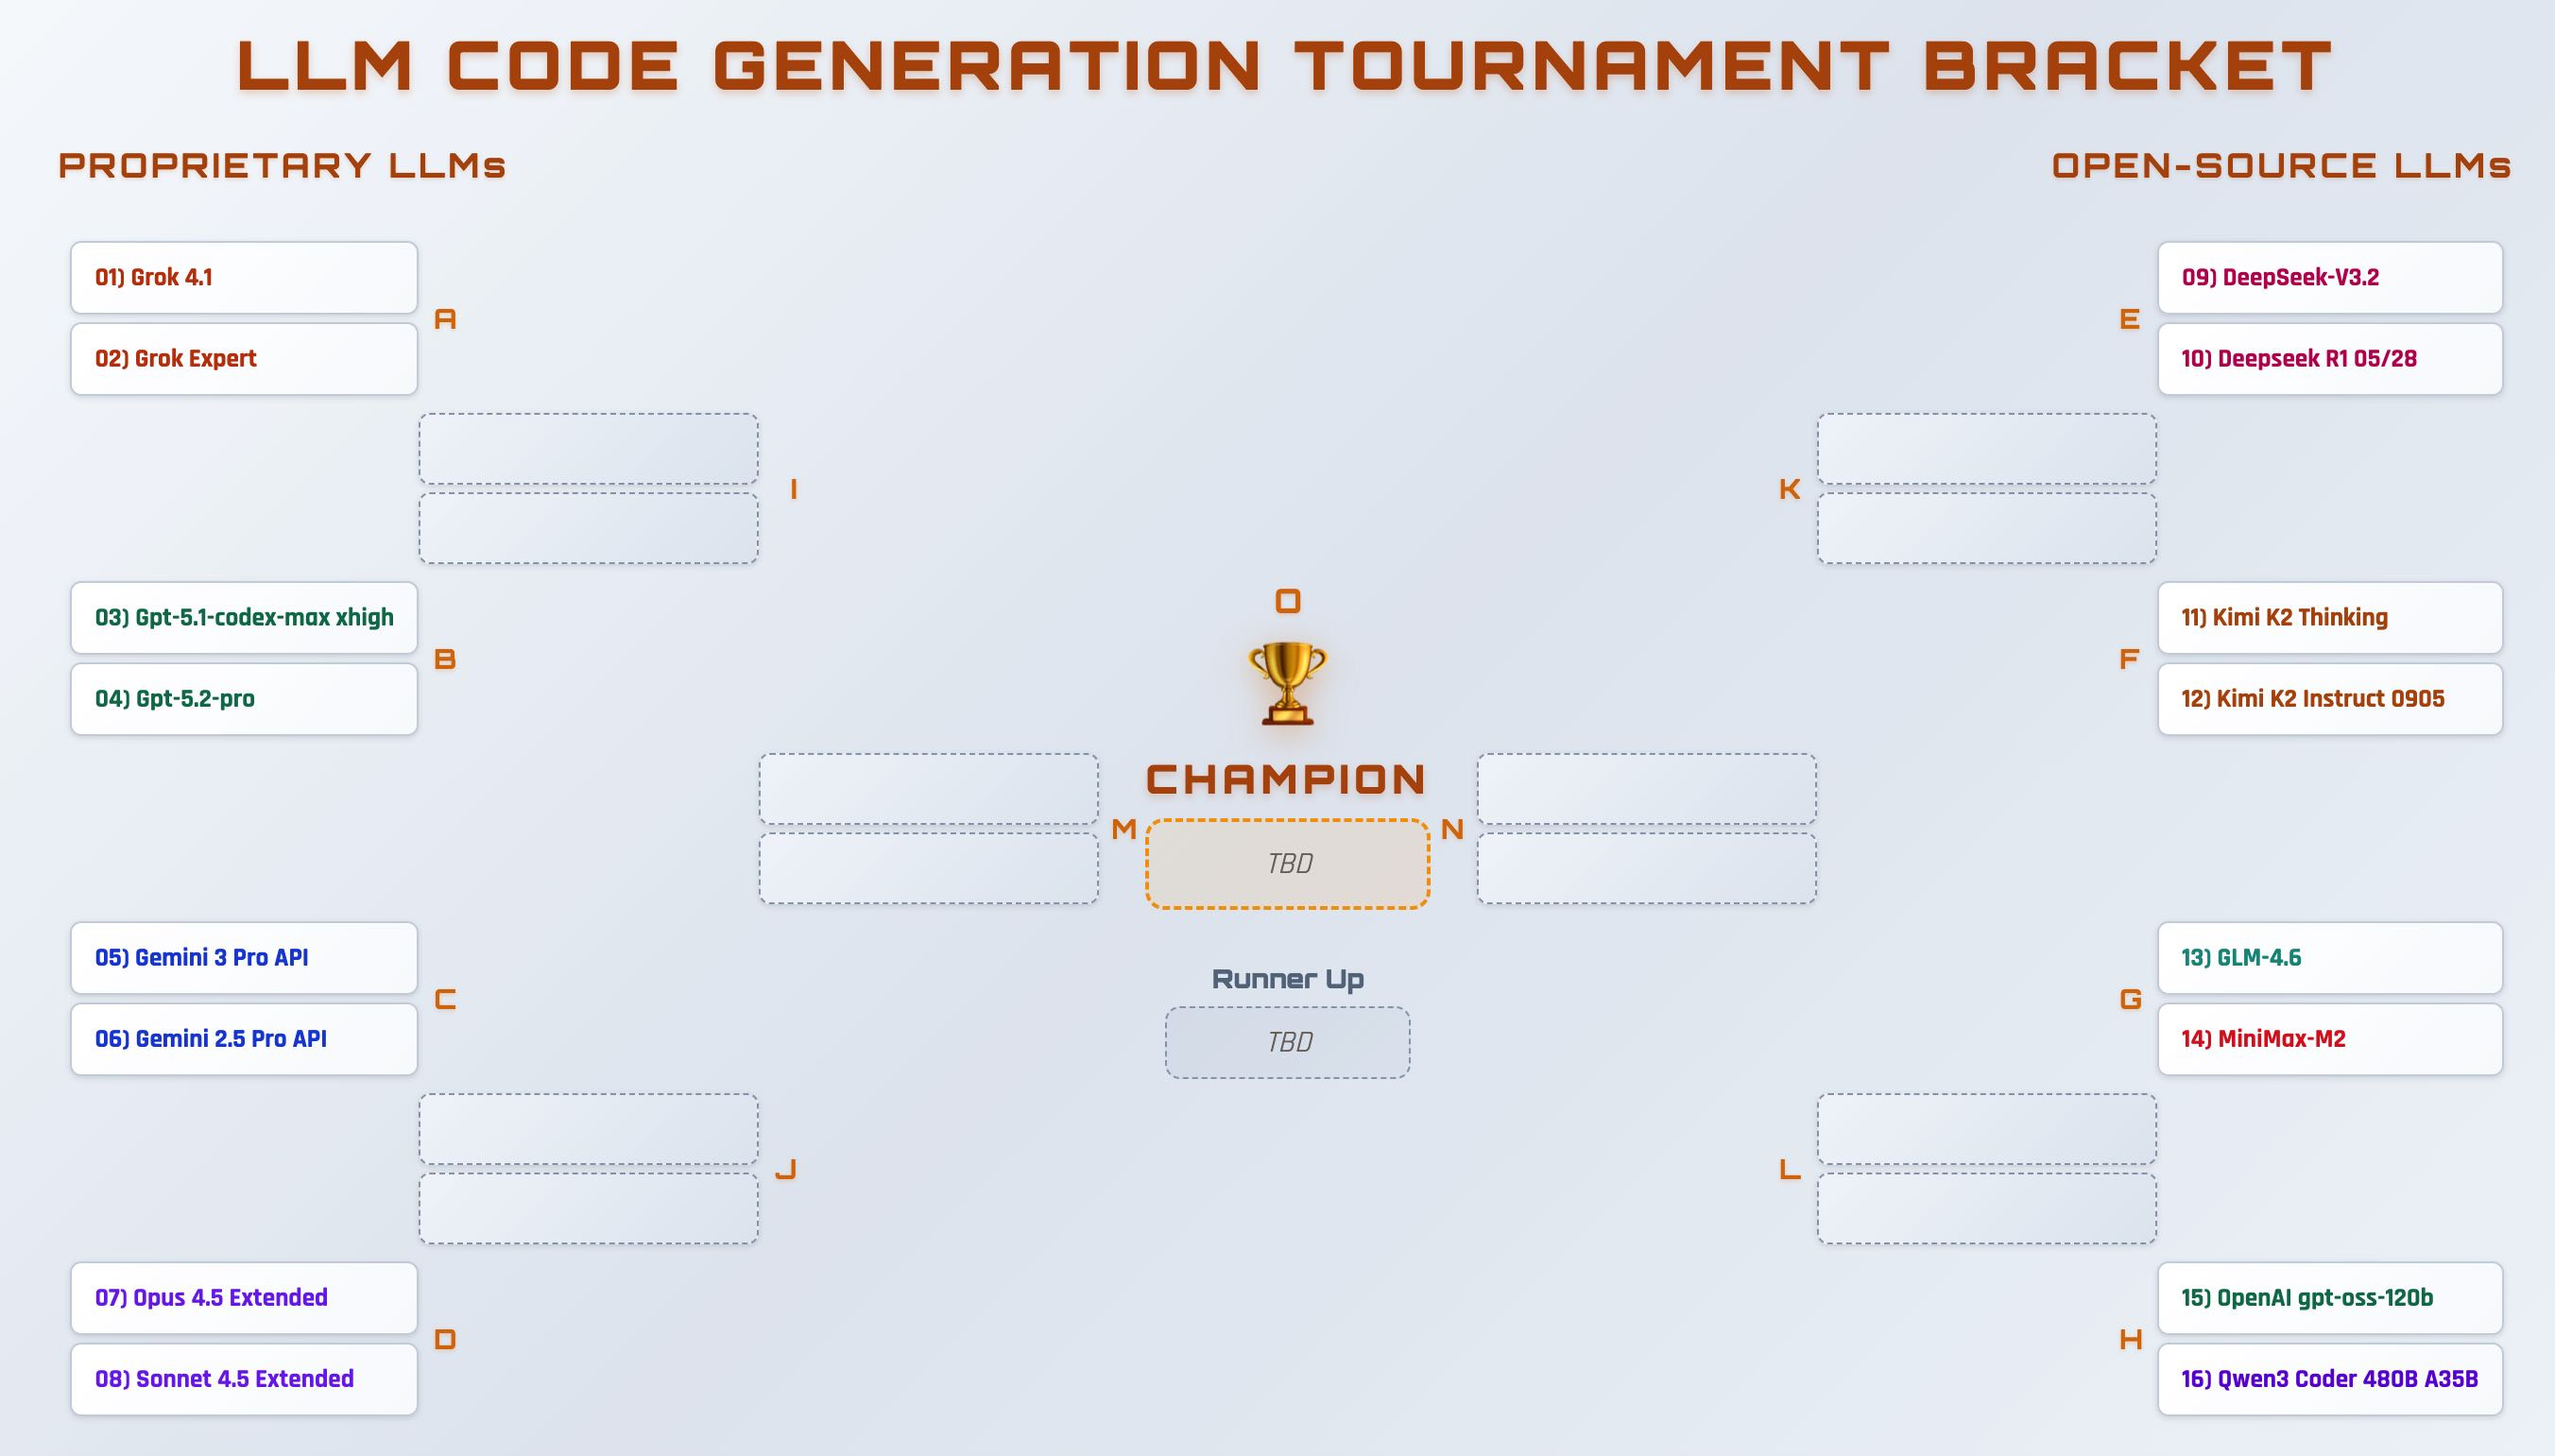
\includegraphics[width=1.0\linewidth, trim={0 0 0 0}, clip]{Images/Bracket_Before.jpg}
    % \vspace{0.1cm}
    \caption{16 LLM Single-Elimination Code Generation Bracket with Iterative Learning\\Process Throughout Rounds Based on FDA Adverse Event Reporting System (FAERS)}
    \label{EntryBracket}
\end{figure}







\begin{minipage}{\textwidth}
\renewcommand{\contentsname}{Table of Contents}
\addtocontents{toc}{\protect\setlength{\parskip}{0.5em}}
% \vspace{0.5cm}
\tableofcontents
\end{minipage}






\vspace{-0.2cm}


\begin{minipage}{\textwidth}
\section{Introduction}

 

\subsection{Human Code Iteration}
 
\hspace{1.3em} Humans have been iterating on code for many decades, continually evolving their techniques to obtain maximum efficiency \cite{04IntroPythonSpeed, 07IntroNagappan}. What started as labor-intensive writing and debugging in low level languages has evolved into higher-level language automation \cite{01IntroAntoniou}. Additionally, interactive debugging and profiling tools have made code iteration cycles faster. For example, a programmer can run a Python script, profile its performance, and identify bottlenecks in seconds. Similarly, a programmer's choice of top performing algorithms or data structures can yield large performance gains. Humans can effectively leverage their understanding of the problem domain and context, iterating through memory analyzers to reduce bloat. For instance, developers systematically optimized the interpreter in version Python 3.11, yielding an average 1.22× speedup over Python 3.10, with some benchmarks running 10–60\% faster \cite{02IntroPython311}.  

\vspace{0.2cm} 
\hspace{1.3em} The 2020s introduced structured productivity frameworks like DevOps Research and Assessment's DORA metrics (Deployment frequency, Lead time, Change failure rate, Mean time to restore) \cite{05IntroDORAmetrics}, and Microsoft's SPACE framework (Satisfaction, Performance, Activity, Communication, Efficiency) \cite{06IntroSPACE}. However, humans have been found to be limited to code review effectiveness peaks at under 400 lines per session \cite{03Intro300Lines}. Global optimization is extremely challenging for humans to perform; and optimizing an entire large codebase or complex system is often beyond what a single human (or team) can manage. 
\vspace{-0.6cm}\\
\begin{itemize} [leftmargin=2.2em, itemsep=0em, topsep=0.95em]
    \item Manual optimization is time-consuming and labor-intensive
    \item Humans tend to stop once “fast enough” performance is reached due to fatigue
    \item Diminishing returns: A lot of effort for small gains in obtaining last 3\% improvement
\end{itemize}

  

 


\subsection{AI Code Iteration}
 
\hspace{1.3em} AI code iteration utilizes automated algorithms or machine intelligence to iteratively refine code. This includes search-based optimization, genetic programming, automated program repair, reinforcement learning, and ML-guided compilers \cite{08IntroAIAlgorithms}. DeepMind's 2022 AlphaTensor project applied reinforcement learning to discover new matrix multiplication algorithms, finding math formulas more efficiently and reducing the number of operations needed \cite{10IntroAlphaTensor, 11IntroATNature}. DeepMind’s 2023 AlphaDev also utilized reinforcement learning in treating algorithm discovery as a game. AlphaDev found new sorting algorithms that surpassed decades-old human benchmarks, and sorting routines were up to 70\% faster for short sequences; while large sequences saw a 1.7\% speed improvement in the C++ standard sorting \cite{09IntroAlphaDev, 12IntroADNature}. Bowtie2 by Langdon, W. et al. optimized the DNA sequence alignment program based on a complex 50,000-line bioinformatics tool. By evolving the C++ code, the AI produced a new version that ran on average 70× faster \cite{13IntroLangdon}. 
 
\vspace{0.2cm} 
\hspace{1.3em} Conversely, AI code iterations are rigid, in that the code must be machine-readable, and the improvement goal must be encoded as a fitness function or reward. This lack of flexibility means these systems only accept certain input formats (e.g. a C++ function plus a test suite). AI systems (pre-LLM) do not provide rationales or high-level explanations for the changes to users; they just output the new code. This opacity means developers might be hesitant to trust and deploy such code. In practice, some AI-discovered solutions have to be carefully reviewed and proved equivalent to the original \cite{14IntroQuantNet}.
\vspace{-0.6cm}\\
\begin{itemize} [leftmargin=2.2em, itemsep=0em, topsep=0.95em]
    \item AI code iteration cannot understanding natural language intent or high-level goals
    \item Concrete metric or formal specification requires expertise for success at scale
    \item AlphaDev required framing as sorting assembly instructions with a defined reward \cite{12IntroADNature}
\end{itemize}


 


\subsection{LLM Code Iteration}
% \vspace{0.2cm} 
\hspace{1.3em} LLM code iteration builds on AI code iteration, but now with mixed language and high contextual awareness capabilities. LLMs have been trained on large portions of internet code and discussions (GitHub repositories \cite{23IntroGitHub}, Stack Overflow Q\&A \cite{24IntroStack}, etc.). DeepMind’s 2025 AlphaEvolve used algorithmic AI agents combining evolutionary search with LLM-guided code generation to iteratively evolve algorithms \cite{21IntroAlphaEvolve, 22IntroAlphaEvolvearXiv}; producing a hashing algorithm 30\% faster than a widely-used human-designed hash. Contemporary Opus 4.5 is “the coding and agentic workflow leader”, scoring 74.4\% on a stringent SWE-bench to iteratively plan, code, and refine \cite{17SWEbenchLead}.

\vspace{0.2cm} 
\hspace{1.3em} OpenAI Gpt-5.2's key strength is speed: Gpt-5.2 processes about 187 tokens/second, which is 3.8× faster than Claude which makes iterations faster \cite{19IntroDigApplied}. Gemini 3 Pro’s focus on multimodal input at 1 million token context window can iterate faster through entire codebases in a single prompt \cite{Gemini3}. The recent DeepSeek V3.2 matches Western models on many benchmarks and boasts much lower cost to make workflows go farther at \$0.56/\$1.68 for 1M input and 1M output vs.\ \$5/\$25 for Opus \cite{Opus45} and \$1.75/\$14.00 for Gpt 5.2 \cite{20IntroOpenAICost} and \$2/\$12 for Gemini 3 \cite{Gemini3}. 
\vspace{-0.6cm}\\
\begin{itemize} [leftmargin=2.2em, itemsep=0em, topsep=0.95em]
    \item LLM interactive prompting and code refinement for generating revised versions
    \item Human in the loop collaboration for effectively noticing a wide range of issues \cite{16IntroMiniMaxIR}
    \item Encyclopedic knowledge of optimization tricks, library functions, and idiomatic improvements
\end{itemize} 


 


 

\end{minipage}




\begin{minipage}{\textwidth}

\vspace{-0.2cm}

\section{Methods}



\textbf{Competition Notebook Development} \normalsize

\hspace{1.3em} The FDA Adverse Event Reporting System (FAERS) July - September 2025 Quarterly ASCII DEMO25Q3.txt, DRUG25Q3.txt, and REAC25Q3.txt data files were utilized in code executions. Opus 4.5 Extended utilized 12 prompts in a single conversation to develop the competition engine shown in Notebook\_Generation. Prompt 01 contained author instructions and data file information to generate a notebook based on "Code\_A" and "Code\_B" competitors. Prompt 02 was aimed at improving Google Drive incorporation; and a sample of the dataset was included to improve applicability.\ ChatGPT 5.1 was utilized to determine 4 larger dataset competition tasks in Prompt 03a/3b \cite{GPT51}. Task A, later renamed Task 1, was ultimately chosen in Prompt 04a as the most relevant to FDA, in regards to LLM code identifying the "First calendar quarters where pair becomes a safety “signal” (PRR \raisebox{0.25ex}{\scalebox{0.7}{$\geq$}} threshold AND count \raisebox{0.25ex}{\scalebox{0.7}{$\geq$}} minimum cases)." Prompt 04 focused further on Task 1, with further competition task optimizations in Prompt 05. Additional improvements were made by Opus regarding the competition task being self contained in Prompt 06; with Output 06 USER\_6th\_FAERS\_LLM\_Competition\_Task1\_v2.ipynb being used in Round 0 LLM code generations.      

\vspace{0.175cm}

\textbf{LLM Competition Code Generations} \normalsize

\hspace{1.3em} Opus was then instructed to design a prompt based on the Output 06 notebook that generated a competition code with the goal of a perfect 1.0 final score based on correctness, methodology, code quality, and algorithmic efficiency, seen in Prompt 07. This prompt was used to assist the author's Round\_1\_Prompt to then generate LLM Round 0 code for 1st Round competition. Additional optimizations afforded an exact competition task; Code A, and Code B answers to Drive were achieved in Prompt 08. The reference solution correctness metric was further optimized in Prompt 09. Opus then recalculated the correctness score of each code submission based on the reference solution in Output 09. Precautions were taken to assure the notebook corresponded to LLM code generation outputs in Prompt 10, which included transitioning to reference-based scoring using pair F1 score, PRR correlation, quarter match, and structure. Errors and Drive issues were fixed in Output 11 and Output 12, with the final Output 12 \_1RD\_Tournament\_FAERS.ipynb being used as the competition engine in Round 1.  

\vspace{0.175cm}
 
\textbf{Rounds 1-4 Code Competition} \normalsize

\hspace{1.3em} First round generated competition code was based on the earlier USER\_6th\_FAERS\_LLM\_Competition\_Task1\_v2.ipynb correctness score calculation, while the newer \_1RD\_Tournament\_FAERS.ipynb was used to generate 2nd round code. Code pairs replaced existing \_1RD\_Tournament\_FAERS.ipynb Section 5 code of each notebook running on a T4 GPU. Model thoughts (if available), outputs, and run times were included in Round\_1.docx. Python notebook JSON code was provided to Gpt and open-source models where file uploads were not allowed. First round pairs A-H yielded 8 scoring results and up to 9 Drive outputs per notebook. Most importantly, 01\_reference\_solution.csv provided the exact 4 line solution, while Code A and Code B outputs either matched or varied from the reference solution. If a function did not execute, no file was outputted for that competitor. The highest LLM total weighted scores from Section 6 advanced to Round 2. Multi\_Round\_Prompt was used for generating Round\_2, Round\_3, and Round\_4 competitor code; which all had minor "instructions for improvement" modifications compared to Round\_1. Rounds 2-4 were run on a v6e-1 TPU, and based on each contestant's prior code competition notebook. For instance, Round 1 winner Grok Expert utilized Multi\_Round\_Prompt and it's prior round A\_1RD\_Tournament\_FAERS.ipynb to generate its Round 2 competitor code; as did Gpt-5.2-pro use Multi\_Round\_Prompt and its B\_1RD\_Tournament\_FAERS.ipynb to generate its Round 2 code. At the end of the 4th round, a champion was determined based on the round's highest total weighted score.               
\vspace{0.175cm}
 


\hspace{1.3em} LaTeX source code, notebook generation inputs \& outputs, competition notebooks for each round, and each round's output are organized in the Data Availability section, and available in supplementary files. The author wrote the abstract, methods, results text, discussion, prompts (except meta prompts), limitations and future work, and conclusion; and was assisted by ChatGPT 5.2 Thinking Deep Research for the introduction. The remaining sections were either derived from data files, notebooks, or generated using LLMs. All visual elements were generated by Opus 4.5 Extended based on result data or notebooks. Google Colab \cite{Google_Colab} was used for notebook code editing, Visual Studio Code \cite{Visual_Studio_Code} was used for code viewing and edits. Google Docs \cite{GoogleDocs} was used for documenting notebook generation inputs, thoughts, and outputs; Docs was also used for managing LLM generated thoughts and code outputs. All open-source models were run in each of the models' Fireworks.ai's "Try" playground page with standard settings, except for a 16,384 Max Tokens modification. All proprietary chat and API playground inference LLMs were executed in MacOS 14.5 (23F79) \cite{macOSSonoma}, Chrome Version 142.0.7444.162 (Official Build) (arm64) \cite{GoogleChrome}. Total AI cost was approximately \$78.06. ChatGPT 5.1 and ChatGPT 5.2 were accessed through the OpenAI Plus plan chat interface as research assistants \cite{GPT51, GPT52}.

\vspace{0.175cm}

\textbf{(8) Proprietary LLMs: Chat/API Playground Interfaces}
\vspace{-0.4cm}\\
\begin{itemize} [leftmargin=1.65em, itemsep=0em, topsep=0.3em]
    \item \textbf{Grok:} xAI Grok 4.1 and Grok Expert were accessed through the SuperGrok website chat interface \cite{Grok41, SuperGrok}
    \item \textbf{Gpt:} Gpt-5.1-codex-max xhigh, Gpt-5.2-pro were accessed through platform.openai.com API "Chat" website \cite{GPT51, GPT52, GPTPlatform}
    \item \textbf{Gemini:} Gemini 3 Pro, 2.5 Pro were accessed through API Key aistudio.google.com. Settings: Temp=1, Thinking level = High (3 Pro), Budget = 32768 (2.5 Pro), Tools = Off, Safety settings = Off, Output length = 65536, Top P = 0.95 \cite{Gemini3, Gemini25, Google_AI_Studio}   
    \item \textbf{Claude:} Opus 4.5 Extended, Sonnet 4.5 Extended were accessed through the Claude Pro plan chat interface \cite{Opus45, Sonnet45, ClaudePro}
\end{itemize}
\textbf{(8) Open Source LLMs: Fireworks AI Defaults \& 16,384 Max Tokens}
\vspace{-0.4cm}\\
\begin{itemize} [leftmargin=1.65em, itemsep=0em, topsep=0.3em]
    \item \textbf{DeepSeek:} DeepSeek-V3.2, R1 05/28 were accessed through the Fireworks.ai inference service \cite{DeepSeekV32, DeepSeekR10528, Fireworks}
    \item \textbf{Kimi:} Kimi K2 Thinking, Instruct 0905 were accessed through the Fireworks.ai inference service \cite{KimiK2Thinking, KimiK2Instruct0905, Fireworks}
    \item \textbf{GLM:} GLM-4.6 was accessed through the Fireworks.ai inference service \cite{GLM46, Fireworks}
    \item \textbf{MiniMax:} MiniMax-M2 was accessed through the Fireworks.ai inference service \cite{MiniMaxM2, Fireworks}
    \item \textbf{OpenAI:} OpenAI gpt-oss-120b was accessed through the Fireworks.ai inference service \cite{gptoss120b, Fireworks}
    \item \textbf{Qwen:} Qwen3 Coder 480B A35B was accessed through the Fireworks.ai inference service \cite{Qwen3Coder480BA35BInstruct, Fireworks}
\end{itemize}
\end{minipage} 

    
    


 


\begin{minipage}{\textwidth}


\section{FDA FAERS Data Files}

\vspace{-0.15cm}
 
\renewcommand{\arraystretch}{1.61}
\setlength{\tabcolsep}{0pt}
\begin{table}[H]
\centering
\begin{tabular}{p{17.8cm}}
\toprule
\centering
\vspace{-0.55cm}
\textbf{FDA Adverse Event Reporting System (FAERS)} \\
\midrule
\vspace{0.055cm}
\\
\raggedright
\fontsize{8.25pt}{9.25pt}\selectfont
\vspace*{0.05cm}
\textbf{DEMO25Q3: Demographic Data, First 3 Entries Shown}\\
\vspace*{-0.005cm}
{\renewcommand{\arraystretch}{1.05}
\begin{tabular}{p{1.6cm} p{1.35cm} p{1.15cm} p{3.0cm} p{0.7cm} p{1.2cm} p{0.6cm} p{0.6cm} p{1.1cm} p{1.3cm} p{1.3cm} p{2.3cm} p{2cm}}
\textbf{primaryid} & \textbf{caseid} & \textbf{i\_f\_code} & \textbf{mfr\_sndr} & \textbf{age} & \textbf{age\_cod} & \textbf{sex} & \textbf{wt} & \textbf{wt\_cod} & \textbf{rept\_cod} & \textbf{occp\_cod} & \textbf{reporter\_country} & \textbf{occr\_country} \\
100289774 & 10028977 & F & GLAXOSMITHKLINE & 53 & YR & M &  &  & EXP & MD & IN & IN\\
1005762123 & 10057621 & F & ROCHE & 57 & YR & M & 53 & KG & EXP & CN & CA & CA\\
1006831310 & 10068313 & F & PFIZER & 69 & YR & F & 72 & KG & PER & CN & US & US\\
\end{tabular}}
\midrule\\ 

\vspace{0.05cm}

\textbf{DRUG25Q3: Drug Information 7 Columns Not Shown}\\
\vspace*{-0.005cm}
{\renewcommand{\arraystretch}{1.05}
\begin{tabular}{p{1.45cm} p{1.35cm} p{1.35cm} p{1.2cm} p{3.7cm} p{3.7cm} p{1.4cm} p{1.45cm} p{1.05cm} p{1.0cm}}
\textbf{primaryid} & \textbf{caseid} & \textbf{drug\_seq} & \textbf{role\_cod} & \textbf{drugname} & \textbf{prod\_ai} & \textbf{route} & \textbf{dose\_vbm} & \textbf{dechal} & \textbf{rechal} \\
100289774 & 10028977 & 1 & PS & DICLOFENAC POTASSIUM & DICLOFENAC POTASSIUM &  & UNK & Y & U\\
100289774 & 10028977 & 2 & C & ONDANSETRON & ONDANSETRON & Unknown & UNK & U & \\
100289774 & 10028977 & 3 & C & TRAMADOL & TRAMADOL & Unknown & UNK & U & \\
\end{tabular}} 
\midrule\\

\vspace{0.05cm}

\textbf{REAC25Q3: Adverse Reactions, Column 4 Fields n/a}\\
\vspace*{-0.005cm}
{\renewcommand{\arraystretch}{1.05}
\begin{tabular}{p{1.5cm} p{1.5cm} p{3.25cm} p{6.0cm}}
\textbf{primaryid} & \textbf{caseid} & \textbf{pt} & \textbf{drug\_rec\_act} \\
100289774 & 10028977 & Fixed eruption & \\
100289774 & 10028977 & Stevens-Johnson syndrome & \\
100289774 & 10028977 & Toxic epidermal necrolysis & \\
\end{tabular}}
\\
\bottomrule
\end{tabular}

\vspace{0.35cm}
\caption{FAERS July - September 2025 Quarterly ASCII Data Files, 3 of 7 \cite{09BodyFAERS}}
\label{RefDS}
\end{table}





\vspace{-0.3cm}
\newlength{\tablewidthA}
\setlength{\tablewidthA}{17.5cm}
\renewcommand{\arraystretch}{1.45}
\setlength{\tabcolsep}{4pt}
\noindent
\begin{tabular}{|p{0.14\tablewidthA}|p{0.20\tablewidthA}|p{0.18\tablewidthA}|p{0.16\tablewidthA}|p{0.12\tablewidthA}|p{0.10\tablewidthA}|}
\hline 
\multicolumn{6}{|c|}{\rule{0pt}{12pt}\textbf{Rounds 1-4 Reference Solution (01\_reference\_solution.csv)}\rule[-6pt]{0pt}{6pt}} \\
\hline
\raggedright\textbf{Drug Name} & \raggedright\textbf{Reaction} & \raggedright\textbf{Emergence Quarter} & \raggedright\textbf{Emergence PRR} & \raggedright\textbf{Total Cases} & \raggedright\arraybackslash\textbf{Is Signal} \\
\hline
\raggedright DUPIXENT & \raggedright Eczema & \raggedright 2025Q1 & \raggedright 5.058 & \raggedright 5 & \raggedright\arraybackslash True \\
\hline
\raggedright DUPIXENT & \raggedright Pruritus & \raggedright 2025Q1 & \raggedright 4.215 & \raggedright 8 & \raggedright\arraybackslash True \\
\hline
\raggedright DUPIXENT & \raggedright Condition aggravated & \raggedright 2025Q1 & \raggedright 3.793 & \raggedright 5 & \raggedright\arraybackslash True \\
\hline
\raggedright DUPIXENT & \raggedright Dyspnoea & \raggedright 2025Q1 & \raggedright 2.529 & \raggedright 5 & \raggedright\arraybackslash True \\
\hline
\end{tabular}
\vspace{-0.1em}
\noindent
\captionof{table}{Reference \& Contestant Goal Output. Drug-Reaction Pairs Derived from DEMO, DRUG, REAC.\\First Calendar Quarters Where Pair Becomes a Signal (PRR \raisebox{0.25ex}{\scalebox{0.7}{$\geq$}} Threshold AND Count \raisebox{0.25ex}{\scalebox{0.7}{$\geq$}} Minimum Cases)}
\label{RefSolution}


\vspace{0.1cm}

\section{Results}


\subsection{FAERS \& Rounds 1-3}

\hspace{1.3em} \autoref{RefDS} above represents a sampling of the static FDA Adverse Event Reporting System (FAERS) dataset used in rounds.\ \autoref{RefSolution} is the final reference solution that each competitor's function was seeking to output.\ After the \_1RD\_Tournament\_FAERS.ipynb was finalized, head-to-head code matchups were conducted for Rounds 1-3, as detailed in the Methods section and in \autoref{NBIntroRounds}.\ The winner of each round's Python notebook was used as the input along with Multi\_Round\_Prompt to enable iterative updates for subsequent rounds.  

\subsection{Round 4 Code Results}
\hspace{1.3em} The 152 line Gpt-5.2-pro Round 4 detect\_signal\_emergence\_improved function, which is based on its prior Round M notebook and Multi\_Round\_Prompt from \autoref{PromptsTab3} is provided in the following page to build drug–reaction pairs and compute PRR-like observed/expected per quarter. The function uses 9 algorithms for data cleaning/schema normalization, rule-based filtering, deterministic time-binning, relational join/entity resolution, frequency counting/contingency component estimation, observed–expected disproportionality, thresholding/decision rule, “first hitting time”/earliest-emergence selection, and post-processing/summarization.  \\
 
\vspace{-0.1cm}

\textbf{Multi\_Round\_Prompt LLM Thoughts Addressed}
\vspace{-0.6cm}\\
\begin{itemize} [leftmargin=0.8em, itemsep=0em, topsep=0.95em] \fontsize{9.5pt}{10.5pt}\selectfont
    \item "Achieving a perfect score of 1.0 on all metrics is the goal"
    \item "To improve the quality from Code\_A’s score of 9.5 to 10 [prior Round 3 notebook's Gpt-5.2-pro code], I should add type hints, enhance docstrings, ensure vectorization, have a function count of at least three, and maintain a proper comment ratio"
    \item "I’m planning to create a function that includes type hints and input checking while avoiding external dependencies"
\end{itemize}

 \textbf{Competition Code Implements Useful Comments}
\vspace{-0.4cm}\\
\begin{enumerate} [leftmargin=1.3em, itemsep=0em, topsep=0.3em] \fontsize{9.5pt}{10.5pt}\selectfont
    \item "Matched the notebook Reference Solution exactly (per-quarter PRR via expected=(drug\_cases*reac\_cases)/total\_cases, earliest-quarter emergence, PRR rounded to 3)."
    \item "Hardened input handling (column normalization, strict FAERS event\_dtquarter parsing, safe early exits with correct empty schema)." 
    \item "Kept performance high and stable (column subsetting, vectorized groupby/nunique + merges; no Python loops over rows)."
\end{enumerate}
\normalsize 



\end{minipage}

\begin{minipage}{\textwidth}


\begin{minipage}{\textwidth}
\vspace{-1.4cm}
% Python code box
\newtcblisting{pythoncode}[1][]{
    listing only,
    breakable=false,  
    listing options={
        language=Python,
        mathescape=false,
        basicstyle=\ttfamily\fontsize{0.1pt}{0.1pt}\selectfont,
        keywordstyle=\color{keywordcolor}\bfseries,
        stringstyle=\color{stringcolor},
        commentstyle=\color{commentcolor}\itshape,
        numbers=none,
        numberstyle=\fontsize{4pt}{4pt}\selectfont\selectfont\color{gray},
        numbersep=1pt,
        breaklines=true,
        % breakatwhitespace=false,
        showstringspaces=false,
        keepspaces=true,
        columns=flexible,
        tabsize=4
    },
    colback=codebg,
    colframe=gray!50,
    arc=2mm,
    boxrule=0.8pt,
    left=3mm,
    right=3mm,
    top=-1mm,
    bottom=-1mm,
    toptitle=0.5mm,
    title={\textbf{Gpt-5.2-pro Round 4 Code Submission, 152 Lines}},
    fonttitle=\scriptsize,
    coltitle=black,
    colbacktitle=gray!20,
    #1
}



\vspace{0.3cm}

\begin{pythoncode}
def detect_signal_emergence_improved(demo_df: pd.DataFrame,
                                    drug_df: pd.DataFrame,
                                    reac_df: pd.DataFrame,
                                    min_cases: int = 3,
                                    prr_threshold: float = 2.0) -> pd.DataFrame:
    """
    Improved implementation of Task 1 (TASK_1_SPEC).

    Improvements made:
    # 1. Matched the notebook Reference Solution exactly (per-quarter PRR via expected=(drug_cases*reac_cases)/total_cases, earliest-quarter emergence, PRR rounded to 3).
    # 2. Hardened input handling (column normalization, strict FAERS event_dt→quarter parsing, safe early exits with correct empty schema).
    # 3. Kept performance high and stable (column subsetting, vectorized groupby/nunique + merges; no Python loops over rows).

    Returns a DataFrame with columns:
    ['drug_name', 'reaction', 'emergence_quarter', 'emergence_prr', 'total_cases', 'is_signal']
    """
    required_out_cols = [
        "drug_name", "reaction", "emergence_quarter",
        "emergence_prr", "total_cases", "is_signal"
    ]

    def _empty() -> pd.DataFrame:
        return pd.DataFrame(columns=required_out_cols)

    def _norm_cols(df: pd.DataFrame) -> pd.DataFrame:
        if df is None or not isinstance(df, pd.DataFrame) or df.empty:
            return pd.DataFrame()
        out = df.copy(deep=False)
        out.columns = out.columns.astype(str).str.lower().str.strip()
        return out

    def _parse_quarter(demo: pd.DataFrame) -> pd.DataFrame:
        # Matches the notebook reference parsing behavior exactly.
        if demo.empty or ("primaryid" not in demo.columns) or ("event_dt" not in demo.columns):
            return pd.DataFrame(columns=["primaryid", "quarter"])

        d = demo[["primaryid", "event_dt"]].dropna(subset=["event_dt"]).copy()
        d["event_dt_str"] = d["event_dt"].astype(str).str.replace(".0", "", regex=False)
        d = d[d["event_dt_str"].str.len() >= 6]

        d["year"] = d["event_dt_str"].str[:4]
        d["month"] = pd.to_numeric(d["event_dt_str"].str[4:6], errors="coerce")
        d = d[d["month"].notna() & d["year"].astype(str).str.match(r"^\d{4}$", na=False)]
        d = d[(d["month"] >= 1) & (d["month"] <= 12)]

        d["quarter"] = d["year"].astype(str) + "Q" + (((d["month"] - 1) // 3 + 1).astype(int)).astype(str)
        return d[["primaryid", "quarter"]]

    # --- Normalize inputs (robust to column casing/whitespace) ---
    demo = _norm_cols(demo_df)
    drug = _norm_cols(drug_df)
    reac = _norm_cols(reac_df)
    if demo.empty or drug.empty or reac.empty:
        return _empty()

    # --- Suspect drug filtering + normalization (uppercase, trimmed) ---
    need_drug_cols = {"primaryid", "drugname", "role_cod"}
    need_reac_cols = {"primaryid", "pt"}
    if not need_drug_cols.issubset(drug.columns) or not need_reac_cols.issubset(reac.columns):
        return _empty()

    drugs = drug.loc[drug["role_cod"].isin(["PS", "SS"]), ["primaryid", "drugname"]].copy()
    if drugs.empty:
        return _empty()
    drugs["drugname"] = drugs["drugname"].astype(str).str.upper().str.strip()

    # --- Parse quarters from DEMO ---
    demo_q = _parse_quarter(demo)
    if demo_q.empty:
        return _empty()

    # --- Merge DRUG + REAC + DEMO on primaryid (inner joins as reference) ---
    merged = (
        drugs.merge(reac[["primaryid", "pt"]], on="primaryid", how="inner")
             .merge(demo_q, on="primaryid", how="inner")
    )
    if merged.empty:
        return _empty()

    # --- Per-quarter component counts (unique primaryid) ---
    quarter_totals = (
        merged.groupby("quarter", sort=False)
              .agg(total_cases=("primaryid", "nunique"))
              .reset_index()
    )
    drug_quarter = (
        merged.groupby(["drugname", "quarter"], sort=False)["primaryid"]
              .nunique()
              .reset_index(name="drug_cases")
    )
    reac_quarter = (
        merged.groupby(["pt", "quarter"], sort=False)["primaryid"]
              .nunique()
              .reset_index(name="reac_cases")
    )
    pair_quarter = (
        merged.groupby(["drugname", "pt", "quarter"], sort=False)["primaryid"]
              .nunique()
              .reset_index(name="pair_cases")
    )

    analysis = (
        pair_quarter.merge(drug_quarter, on=["drugname", "quarter"], how="left")
                    .merge(reac_quarter, on=["pt", "quarter"], how="left")
                    .merge(quarter_totals, on="quarter", how="left")
    )

    # Reference PRR definition used in notebook:
    # expected = (drug_cases * reac_cases) / total_cases ; prr = pair_cases / expected
    analysis["expected"] = (analysis["drug_cases"] * analysis["reac_cases"]) / analysis["total_cases"]
    analysis["prr"] = np.where(analysis["expected"] > 0, analysis["pair_cases"] / analysis["expected"], 0.0)

    # --- Signal emergence (first quarter meeting threshold) ---
    signals = analysis[
        (analysis["prr"] >= float(prr_threshold)) & (analysis["pair_cases"] >= int(min_cases))
    ].copy()
    if signals.empty:
        return _empty()

    signals = signals.sort_values("quarter", ascending=True)
    first_emergence = signals.groupby(["drugname", "pt"]).first().reset_index()

    total_by_pair = (
        merged.groupby(["drugname", "pt"], sort=False)["primaryid"]
              .nunique()
              .reset_index(name="total_cases_all")
    )

    result_df = first_emergence[["drugname", "pt", "quarter", "prr"]].merge(
        total_by_pair, on=["drugname", "pt"], how="left"
    )

    result_df = result_df.rename(columns={
        "drugname": "drug_name",
        "pt": "reaction",
        "quarter": "emergence_quarter",
        "prr": "emergence_prr",
        "total_cases_all": "total_cases",
    })
    result_df["emergence_prr"] = result_df["emergence_prr"].astype(float).round(3)
    result_df["total_cases"] = result_df["total_cases"].fillna(0).astype(int)
    result_df["is_signal"] = True

    return (
        result_df[required_out_cols]
        .sort_values("emergence_prr", ascending=False)
        .reset_index(drop=True)
    )

# REQUIRED: Set result variable
result = detect_signal_emergence_improved(demo_df, drug_df, reac_df)
print(f"Found {len(result)} signals")
\end{pythoncode}
% \captionof{figure}{Drug Synergy Dataset Import and Initial Preview}
\label{GPT52ProCode}
\end{minipage}



\end{minipage}




\begin{minipage}{\textwidth}

\subsection{Round 4 Notebook Results}

\hspace{1.3em} The notebook introduction shown in \autoref{NBIntroRounds} provides the cross-table temporal signal emergence detection competition task, scoring system, and output structure. It is important to note that correctness is based on a head-to-head comparison to 01\_reference\_solution.csv shown in \autoref{RefSolution}. The following \autoref{HeadToHeadRound4} shows time, speed, and cost benefits favoring the open-source gpt-oss-120b over the proprietary Gpt-5.2-pro. It was significant that the three Gpt-5.2-pro helper functions contributed to higher Code Quality score (0.95 vs. 0.90) and decisive error handling. The Round 4 results output provides each of the four reference-based scoring metrics (correctness, methodology, code quality, and algorithmic efficiency) of Code\_A (Gpt-5.2-pro) and Code\_B (OpenAl gpt-oss-120b) in \autoref{OutputChampRound}. Gpt-5.2-pro (0.9775/1.0) correctness matched the reference solution (1.0/1.0), with a top methodology score (1.0/1.0); while OpenAl gpt-oss-120b (0.2050/1.0) failed to execute, but had a code quality score of 9.0/10. The multi-metric score framework is illustrated in \autoref{ScoringWheel} and itemized with final weighted scores in \autoref{MetricCorrectness}-\autoref{MetricFinalWeighted}.




\begin{figure}[H]
    \raggedright
    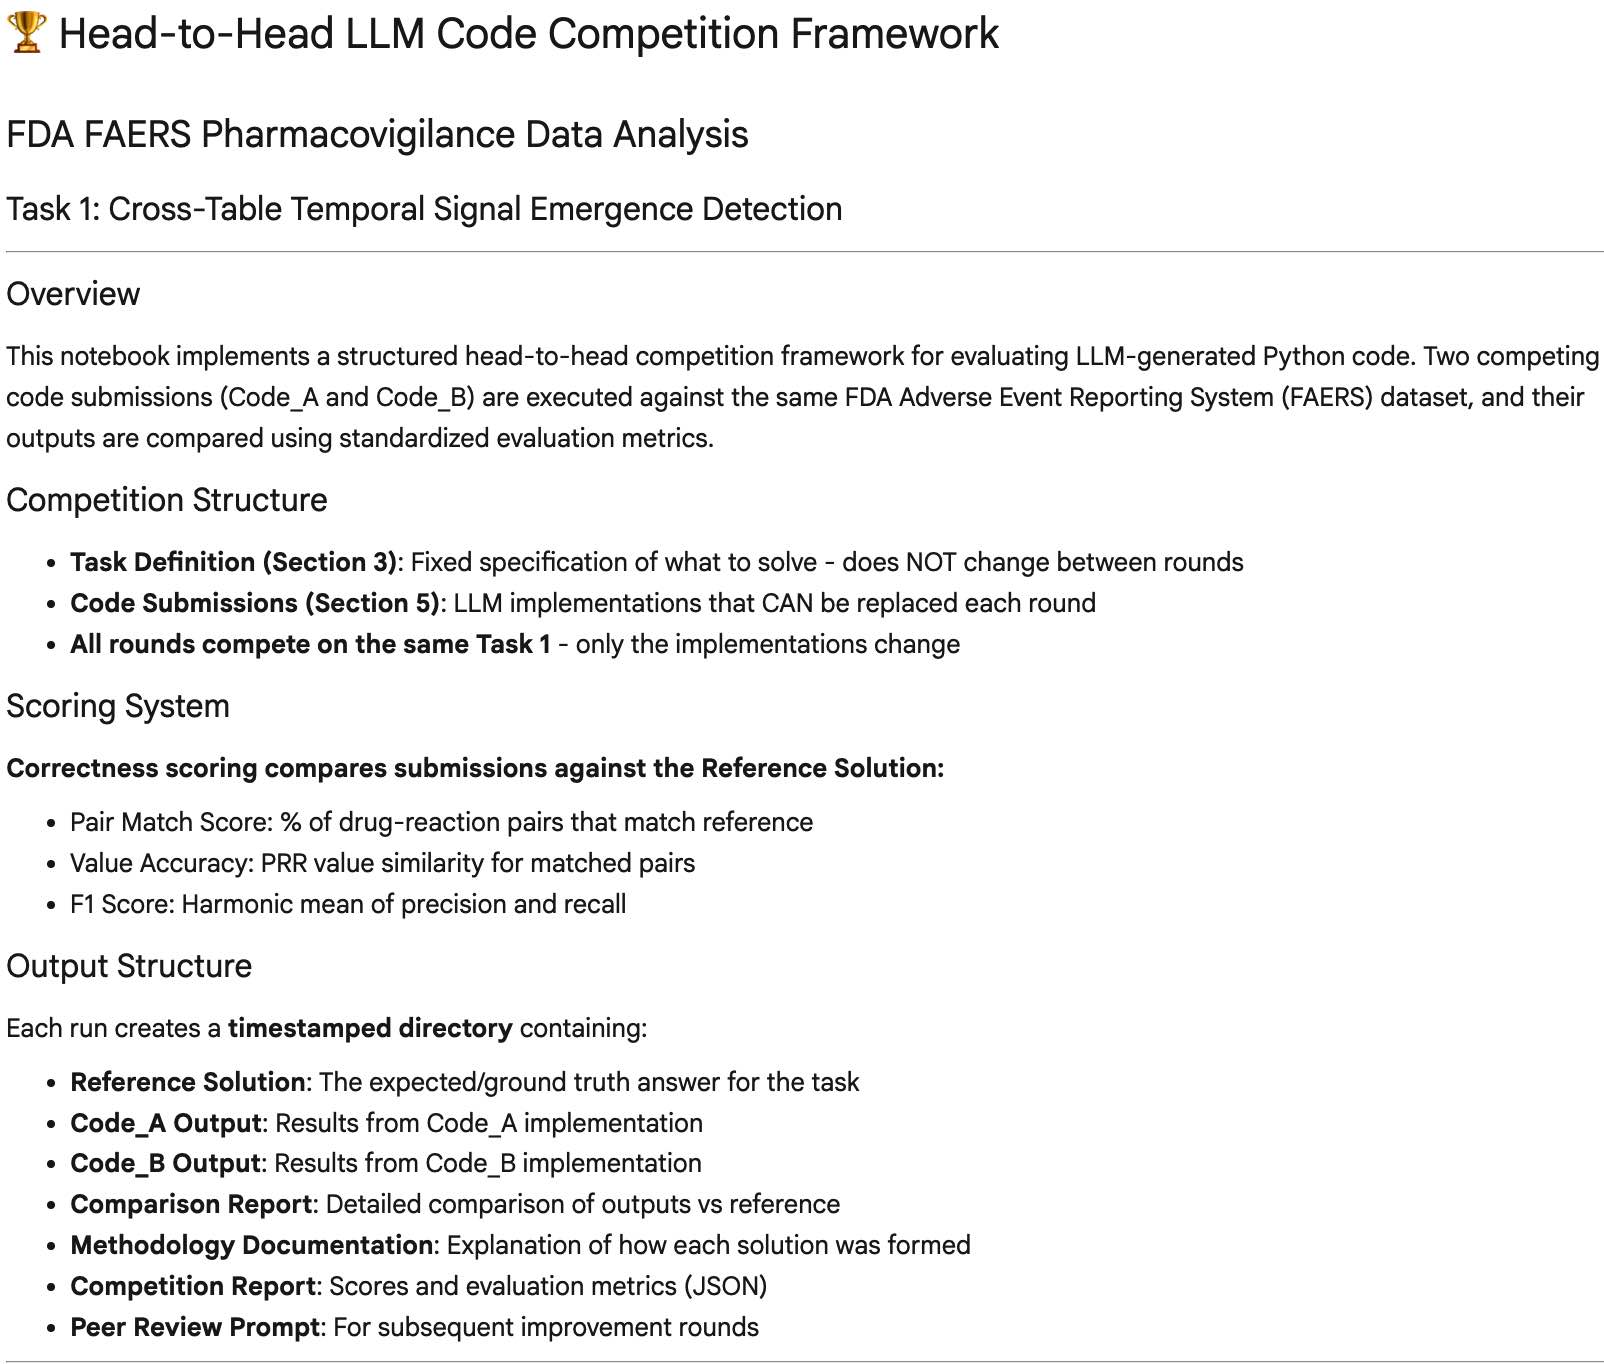
\includegraphics[width=1.0\linewidth, trim={0 0 0 0}, clip]{Images/Round4Notebook.jpg}
    % \vspace{0.1cm}
    \caption{Rounds 1-4 Competition Notebook Screenshot}
    \label{NBIntroRounds}
\end{figure}

\end{minipage}








\begin{minipage}{\textwidth}

 
\vspace{0.4cm}

\newlength{\tablewidthL}
\setlength{\tablewidthL}{18.1cm}

\renewcommand{\arraystretch}{1.45}
\setlength{\tabcolsep}{4pt}

\noindent
\begin{tabular}{|p{0.24\tablewidthL}|p{0.39\tablewidthL}|p{0.31\tablewidthL}|}
\hline
\multicolumn{3}{|c|}{\rule{0pt}{12pt}\textbf{Round 4 Code Generation Metrics (Single Iteration)}\rule[-6pt]{0pt}{6pt}} \\
\hline
\raggedright\textbf{Metric} & \raggedright\textbf{Gpt-5.2-pro} & \raggedright\arraybackslash\textbf{gpt-oss-120b} \\
\hline
\raggedright Generation Time & \raggedright 2 min 49.37 sec & \raggedright\arraybackslash 0 min 25.65 sec \\
\hline
\raggedright Generation Speed & \raggedright \raisebox{0.1ex}\textasciitilde 19.5 tokens/sec & \raggedright\arraybackslash 122.34 tokens/sec \\
\hline
\raggedright Generation Cost & \raggedright \$1.42 & \raggedright\arraybackslash \$0.01 \\
\hline
\raggedright Output Tokens & \raggedright 3,292 T & \raggedright\arraybackslash \raisebox{0.1ex}\textasciitilde3,134 T (est.) \\
\hline
\raggedright Input Tokens & \raggedright 46.8 KT & \raggedright\arraybackslash \raisebox{0.1ex}\textasciitilde41.6 KT (est.) \\
\hline
\raggedright Lines of Code & \raggedright 127 LOC & \raggedright\arraybackslash 142 LOC \\
\hline
\raggedright Helper Functions & \raggedright 3 (\_empty, \_norm\_cols, \_parse\_quarter) & \raggedright\arraybackslash 0 (inline logic only) \\
\hline
\end{tabular}
\vspace{-0.1em}
\noindent
{\captionsetup{width=\tablewidthCorr}
\captionof{table}{Proprietary vs.\ Open-Source Model Differences}
\label{HeadToHeadRound4}
 

\vspace{1cm}

\vspace{-1cm}
 
\newtcblisting{outputbox}[1][]{
    listing only,
    breakable=false,
    listing options={
        basicstyle=\ttfamily\bfseries\scriptsize,  % Added \bfseries here
        escapeinside={(*@}{@*)},
        breaklines=true,
        showstringspaces=false,
        keepspaces=true,
        columns=flexible
    },
    colback=codebg,
    colframe=gray!50,
    arc=2mm,
    boxrule=0.8pt,
    left=3mm,
    right=3mm,
    top=-1mm,
    bottom=-1mm,
    toptitle=0.5mm,
    title={\textbf{Round 4 Results. Code\_A = Gpt-5.2-pro. Code\_B = OpenAl gpt-oss-120b}},
    fonttitle=\small,
    coltitle=black,
    colbacktitle=gray!20,
    #1
}

\vspace{0.3cm}
\begin{outputbox}
======================================================================
(*@\faGamepad@*) STARTING HEAD-TO-HEAD COMPETITION
======================================================================
Competition ID: FAERS_25Q3_COMPETITION
Task: Task 1: Cross-Table Temporal Signal Emergence Detection
Data Sample: 10%
Reference Solution: 4 signals
Output Directory: /content/drive/MyDrive/Colab Notebooks/Inputs/FAERS_LLM_Competition/results/run_20251212_215200
======================================================================
(*@\faFlagCheckered@*) COMPETITION ROUND: T1_TEMPORAL_SIGNAL_R1_038e016e
   Task: Task 1: Cross-Table Temporal Signal Emergence Detection
   Reference Solution: 4 signals
======================================================================
   Code_A hash: 9838497cf082
   Code_B hash: ce3db45a915c
(*@\faMapMarkerAlt@*) Executing Code_A...
   Runtime: 0.123s | Success: True
   Output: 4 rows
(*@\faMapMarkerAlt@*) Executing Code_B...
   Runtime: 0.001s | Success: False
======================================================================
(*@\faChartBar@*) ROUND RESULTS (Reference-Based Scoring)
======================================================================
   Code_A Score: 0.9775 (*@\textcolor{green!60!black}{\faCheckCircle}@*)
      Correctness:           1.0000 (×0.45)
         ├─ Pair F1:         1.0000 (P:1.00 R:1.00)
         ├─ PRR Correlation:  1.0000
         ├─ Quarter Match:    1.0000
         └─ Matched Pairs:    4/4
      Methodology:           1.0000 (×0.30)
      Code Quality:          9.50/10 (×0.15)
      Algorithmic Effic.:    0.8500 (×0.10)
   Code_B Score: 0.2050 (*@\textcolor{red!70!black}{\faTimesCircle}@*) FAILED
      Correctness:           0.0000 (×0.45)
         ├─ Pair F1:         0.0000 (P:0.00 R:0.00)
         ├─ PRR Correlation:  0.0000
         ├─ Quarter Match:    0.0000
         └─ Matched Pairs:    0/0
      Methodology:           0.0000 (×0.30)
      Code Quality:          9.00/10 (×0.15)
      Algorithmic Effic.:    0.7000 (×0.10)
(*@\faTrophy@*) WINNER: Code_A
======================================================================
\end{outputbox}
\vspace{-0.15cm}
\caption{Round 4 Competition Notebook Section 6.1 Results}
\label{OutputChampRound}


\end{minipage}



\begin{minipage}{\textwidth}

 

\subsection{Reference-Based Scoring Metrics}

\vspace{-0.1cm}

\begin{figure}[H]
    \centering 
    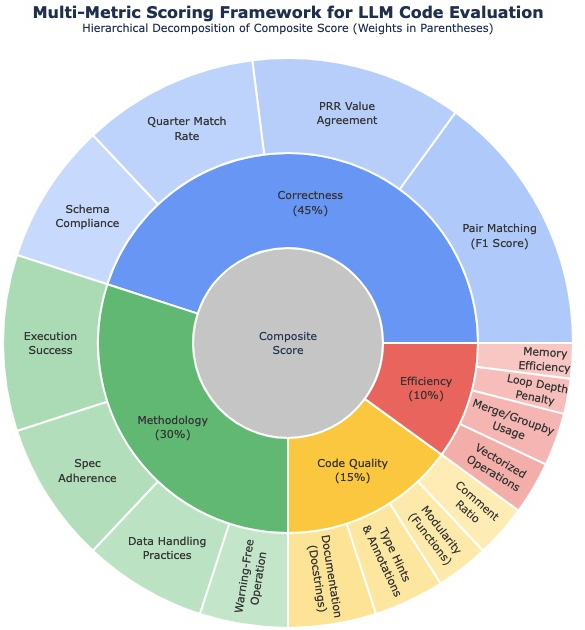
\includegraphics[width=0.525\linewidth, trim={0 0 0 0}, clip]{Images/Framework_Score.jpg}
    % \vspace{0.1cm}
    \caption{Reference-Based Weighted Scoring System}
    \label{ScoringWheel}
\end{figure}

 
 

\newlength{\tablewidthCorr}
\setlength{\tablewidthCorr}{17.5cm}

\renewcommand{\arraystretch}{1.45}
\setlength{\tabcolsep}{4pt}

\noindent
\begin{tabular}{|p{0.25\tablewidthCorr}|p{0.10\tablewidthCorr}|p{0.15\tablewidthCorr}|p{0.15\tablewidthCorr}|p{0.26\tablewidthCorr}|}
\hline
\multicolumn{5}{|c|}{\rule{0pt}{12pt}\textbf{Correctness Scoring Breakdown (45\% Weight)}\rule[-6pt]{0pt}{6pt}} \\
\hline
\raggedright\textbf{Subcategory} & \raggedright\textbf{Weight} & \raggedright\textbf{Gpt-5.2-pro} & \raggedright\textbf{gpt-oss-120b} & \raggedright\arraybackslash\textbf{Assessment Method} \\
\hline
\raggedright Pair F1 Score & \raggedright 40\% & \raggedright 1.0000 & \raggedright 0.0000 & \raggedright\arraybackslash Precision/Recall of pairs \\
\hline
\raggedright PRR Correlation & \raggedright 30\% & \raggedright 1.0000 & \raggedright 0.0000 & \raggedright\arraybackslash Pearson correlation \\
\hline
\raggedright Quarter Match Rate & \raggedright 20\% & \raggedright 1.0000 & \raggedright 0.0000 & \raggedright\arraybackslash Emergence quarter match \\
\hline
\raggedright Structure Score & \raggedright 10\% & \raggedright 1.0000 & \raggedright 0.0000 & \raggedright\arraybackslash Column schema compliance \\
\hline
\raggedright\textbf{CORRECTNESS TOTAL} & \raggedright\textbf{100\%} & \raggedright\textbf{1.0000} & \raggedright\textbf{0.0000} & \raggedright\arraybackslash\textbf{Sum of weighted scores} \\
\hline
\raggedright\textbf{Contribution to Final} & \raggedright\textbf{$\times$0.45} & \raggedright\textbf{0.4500} & \raggedright\textbf{0.0000} & \raggedright\arraybackslash\textbf{Correctness $\times$ 0.45} \\
\hline
\end{tabular}

\vspace{-0.1em}
\noindent
{\captionsetup{width=\tablewidthCorr}
\captionof{table}{Correctness Scoring Formula = $0.40 \times F_1 + 0.30 \times r_{\text{PRR}} + 0.20 \times Q_{\text{match}} + 0.10 \times S_{\text{struct}}$}
\label{MetricCorrectness}






\vspace{0.3cm}

\newlength{\tablewidthMeth}
\setlength{\tablewidthMeth}{17.5cm}

\renewcommand{\arraystretch}{1.45}
\setlength{\tabcolsep}{4pt}

\noindent
\begin{tabular}{|p{0.25\tablewidthCorr}|p{0.10\tablewidthCorr}|p{0.15\tablewidthCorr}|p{0.15\tablewidthCorr}|p{0.26\tablewidthCorr}|}
\hline
\multicolumn{5}{|c|}{\rule{0pt}{12pt}\textbf{Methodology Scoring Breakdown (30\% Weight)}\rule[-6pt]{0pt}{6pt}} \\
\hline
\raggedright\textbf{Subcategory} & \raggedright\textbf{Points} & \raggedright\textbf{Gpt-5.2-pro} & \raggedright\textbf{gpt-oss-120b} & \raggedright\arraybackslash\textbf{Assessment Criterion} \\
\hline
\raggedright Execution Success (Base) & \raggedright +0.70 & \raggedright$\checkmark$ +0.70 & \raggedright\ding{55} +0.00 & \raggedright\arraybackslash Error-free execution \\
\hline
\raggedright Warning Penalty & \raggedright --0.10 each & \raggedright 0 warnings & \raggedright N/A (failed) & \raggedright\arraybackslash Max --0.30 for 3+ warnings \\
\hline
\raggedright Vectorized Operations & \raggedright +0.10 & \raggedright$\checkmark$ +0.10 & \raggedright N/A (failed) & \raggedright\arraybackslash Uses np.*, .str., .dt. \\
\hline
\raggedright Function Count $\geq$ 2 & \raggedright +0.10 & \raggedright$\checkmark$ +0.10 & \raggedright N/A (failed) & \raggedright\arraybackslash Modular code structure \\
\hline
\raggedright Has Docstrings & \raggedright +0.10 & \raggedright$\checkmark$ +0.10 & \raggedright N/A (failed) & \raggedright\arraybackslash Triple-quote documentation \\
\hline
\raggedright\textbf{METHODOLOGY TOTAL} & \raggedright\textbf{max 1.0} & \raggedright\textbf{1.0000} & \raggedright\textbf{0.0000} & \raggedright\arraybackslash\textbf{Capped at 1.0} \\
\hline
\raggedright\textbf{Contribution to Final} & \raggedright\textbf{$\times$0.30} & \raggedright\textbf{0.3000} & \raggedright\textbf{0.0000} & \raggedright\arraybackslash\textbf{Methodology $\times$ 0.30} \\
\hline
\end{tabular}

\vspace{-0.1em}
\noindent
{\captionsetup{width=\tablewidthCorr}
\captionof{table}{Methodology Based on Execution Success, Code Practices. Base = 0.70 + (3) +0.10 Bonuses}
\label{MetricMethodology}



\end{minipage}

\vspace{1.5em}

 
\begin{minipage}{\textwidth}
\vspace{-0.3cm}

\newlength{\tablewidthQual}
\setlength{\tablewidthQual}{17.5cm}

\renewcommand{\arraystretch}{1.45}
\setlength{\tabcolsep}{4pt}

\noindent
\begin{tabular}{|p{0.25\tablewidthQual}|p{0.1\tablewidthQual}|p{0.15\tablewidthQual}|p{0.15\tablewidthQual}|p{0.26\tablewidthQual}|}
\hline
\multicolumn{5}{|c|}{\rule{0pt}{12pt}\textbf{Code Quality Scoring Breakdown (15\% Weight)}\rule[-6pt]{0pt}{6pt}} \\
\hline
\raggedright\textbf{Subcategory} & \raggedright\textbf{Points} & \raggedright\textbf{Gpt-5.2-pro} & \raggedright\textbf{gpt-oss-120b} & \raggedright\arraybackslash\textbf{Detection Method} \\
\hline
\raggedright Base Score & \raggedright +5.00 & \raggedright +5.00 & \raggedright +5.00 & \raggedright\arraybackslash All submissions start here \\
\hline
\raggedright Has Docstrings & \raggedright +1.50 & \raggedright$\checkmark$ +1.50 & \raggedright$\checkmark$ +1.50 & \raggedright\arraybackslash \texttt{"""} or \texttt{'''} present \\
\hline
\raggedright Has Type Hints & \raggedright +0.50 & \raggedright$\checkmark$ +0.50 & \raggedright$\checkmark$ +0.50 & \raggedright\arraybackslash \texttt{def func(x: Type)} \\
\hline
\raggedright Uses Vectorized Ops & \raggedright +1.00 & \raggedright$\checkmark$ +1.00 & \raggedright$\checkmark$ +1.00 & \raggedright\arraybackslash np.*, .str., .dt., .agg() \\
\hline
\raggedright Function Count $\geq$ 1 & \raggedright +0.50 & \raggedright$\checkmark$ +0.50 & \raggedright$\checkmark$ +0.50 & \raggedright\arraybackslash At least one \texttt{def} \\
\hline
\raggedright Function Count $\geq$ 3 & \raggedright +0.50 & \raggedright$\checkmark$ +0.50 & \raggedright\ding{55} +0.00 & \raggedright\arraybackslash Three or more \texttt{def} \\
\hline
\raggedright Comment Ratio 10--30\% & \raggedright +0.50 & \raggedright$\checkmark$ +0.50 & \raggedright$\checkmark$ +0.50 & \raggedright\arraybackslash \# lines / code lines \\
\hline
\raggedright\textbf{CODE QUALITY TOTAL} & \raggedright\textbf{/10} & \raggedright\textbf{9.50} & \raggedright\textbf{9.00} & \raggedright\arraybackslash\textbf{Capped at 10.0} \\
\hline
\raggedright\textbf{Contribution to Final} & \raggedright\textbf{$\times$0.015} & \raggedright\textbf{0.1425} & \raggedright\textbf{0.1350} & \raggedright\arraybackslash\textbf{(Quality/10) $\times$ 0.15} \\
\hline
\end{tabular}

\vspace{-0.1em}
\noindent
{\captionsetup{width=\tablewidthCorr}
\captionof{table}{Quality Scoring via Static Analysis, \raisebox{0.25ex}{\scalebox{0.7}{$\geq$}}3 Helper Functions = Bonus}}
\label{MetricCodeQuality}


\end{minipage}

\vspace{1.5em}



 
\begin{minipage}{\textwidth}
\vspace{-0.3cm}

\newlength{\tablewidthEff}
\setlength{\tablewidthEff}{17.5cm}

\renewcommand{\arraystretch}{1.45}
\setlength{\tabcolsep}{4pt}

\noindent
\begin{tabular}{|p{0.25\tablewidthEff}|p{0.1\tablewidthEff}|p{0.15\tablewidthEff}|p{0.15\tablewidthEff}|p{0.26\tablewidthEff}|}
\hline
\multicolumn{5}{|c|}{\rule{0pt}{12pt}\textbf{Algorithmic Efficiency Scoring Breakdown (10\% Weight)}\rule[-6pt]{0pt}{6pt}} \\
\hline
\raggedright\textbf{Subcategory} & \raggedright\textbf{Points} & \raggedright\textbf{Gpt-5.2-pro} & \raggedright\textbf{gpt-oss-120b} & \raggedright\arraybackslash\textbf{Detection Pattern} \\
\hline
\raggedright Base Score & \raggedright +0.50 & \raggedright +0.50 & \raggedright +0.50 & \raggedright\arraybackslash All submissions start here \\
\hline
\raggedright Uses Vectorized Ops & \raggedright +0.15 & \raggedright$\checkmark$ +0.15 & \raggedright$\checkmark$ +0.15 & \raggedright\arraybackslash np.where, .str., .dt. \\
\hline
\raggedright Uses Merge/Join & \raggedright +0.10 & \raggedright$\checkmark$ +0.10 & \raggedright$\checkmark$ +0.10 & \raggedright\arraybackslash .merge() or .join() \\
\hline
\raggedright Uses GroupBy & \raggedright +0.10 & \raggedright$\checkmark$ +0.10 & \raggedright$\checkmark$ +0.10 & \raggedright\arraybackslash .groupby() \\
\hline
\raggedright Nested Loops $\geq$ 2 & \raggedright --0.15 & \raggedright$\checkmark$ --0.00 & \raggedright\ding{55} --0.15 & \raggedright\arraybackslash Indent-based detection \\
\hline
\raggedright Nested Loops $\geq$ 3 & \raggedright --0.20 & \raggedright$\checkmark$ --0.00 & \raggedright$\checkmark$ --0.00 & \raggedright\arraybackslash Deep nesting penalty \\
\hline
\raggedright\textbf{EFFICIENCY TOTAL} & \raggedright\textbf{max 1.0} & \raggedright\textbf{0.8500} & \raggedright\textbf{0.7000} & \raggedright\arraybackslash\textbf{Clamped [0.0, 1.0]} \\
\hline
\raggedright\textbf{Contribution to Final} & \raggedright\textbf{$\times$0.10} & \raggedright\textbf{0.0850} & \raggedright\textbf{0.0700} & \raggedright\arraybackslash\textbf{Efficiency $\times$ 0.10} \\
\hline
\end{tabular}

\vspace{-0.1em}
\noindent
{\captionsetup{width=\tablewidthCorr}
\captionof{table}{Algorithmic Efficiency via Static Code Analysis: \raisebox{0.25ex}{\scalebox{0.7}{$\geq$}}2 Nested Loops = Penalty}
\label{Metric_AlgorithmicEfficiency}



\vspace{0.3cm}

\newlength{\tablewidthFinal}
\setlength{\tablewidthFinal}{17.5cm}

\renewcommand{\arraystretch}{1.45}
\setlength{\tabcolsep}{4pt}

\noindent
\begin{tabular}{|p{0.25\tablewidthFinal}|p{0.1\tablewidthFinal}|p{0.15\tablewidthFinal}|p{0.15\tablewidthFinal}|p{0.26\tablewidthFinal}|}
\hline
\multicolumn{5}{|c|}{\rule{0pt}{12pt}\textbf{Final Weighted Score Summary (Round 4)}\rule[-6pt]{0pt}{6pt}} \\
\hline
\raggedright\textbf{Metric} & \raggedright\textbf{Weight} & \raggedright\textbf{Gpt-5.2-pro} & \raggedright\textbf{gpt-oss-120b} & \raggedright\arraybackslash\textbf{Weighted Contribution} \\
\hline
\raggedright Correctness & \raggedright 45\% & \raggedright 1.0000 & \raggedright 0.0000 & \raggedright\arraybackslash 0.4500 vs.\ 0.0000 \\
\hline
\raggedright Methodology & \raggedright 30\% & \raggedright 1.0000 & \raggedright 0.0000 & \raggedright\arraybackslash 0.3000 vs.\ 0.0000 \\
\hline
\raggedright Code Quality & \raggedright 15\% & \raggedright 9.50/10 & \raggedright 9.00/10 & \raggedright\arraybackslash 0.1425 vs.\ 0.1350 \\
\hline
\raggedright Alg.\ Efficiency & \raggedright 10\% & \raggedright 0.8500 & \raggedright 0.7000 & \raggedright\arraybackslash 0.0850 vs.\ 0.0700 \\
\hline
\multicolumn{5}{|c|}{\rule{0pt}{12pt}\textbf{Final Calculation}\rule[-6pt]{0pt}{6pt}} \\
\hline
\raggedright $\sum$ Weighted Scores & \raggedright\textbf{100\%} & \raggedright\textbf{0.9775} & \raggedright\textbf{0.2050} & \raggedright\arraybackslash — \\
\hline
\raggedright Score Differential & \raggedright — & \multicolumn{2}{c|}{\raggedright +0.7725 (Gpt-5.2-pro advantage)} & \raggedright\arraybackslash 77.25\% margin \\
\hline
\raggedright\textbf{WINNER} & \raggedright — & \multicolumn{3}{c|}{\raggedright\arraybackslash\textbf{Gpt-5.2-pro (Code\_A Submission)}} \\
\hline
\end{tabular}

\vspace{-0.1em}
\noindent
{\captionsetup{width=\tablewidthCorr}
\captionof{table}{Weighted Score Aggregation Sums Prior Tables' Metrics}
\label{MetricFinalWeighted}


\end{minipage}

\vspace{1.5em}

 
\begin{minipage}{\textwidth}
 

\subsection{Round 4 Final Results}

\hspace{1.3em} The Kimi K2 Thinking purple bubble in \autoref{ScoreImprovementKimi} indicates the largest round improvement, but Gemini 2.5 Pro API, DeepSeek R1 05/28, and GPT-5.2-pro all started with higher initial scores. GPT-5.2-pro won the most rounds, represented by the largest bubble size. \autoref{ScoreProgressionChampion} illustrates score progression throughout the full 4 rounds, with GPT-5.2-pro improving after the first iteration and maintaining it's lead throughout the tournament. OpenAI gpt-oss-120b achieved the highest first round score at 0.9400, which was maintained for two additional rounds, but its code failed to execute in the final round - represented by the late orange line decline. Gemini 2.5 Pro API also improved after the first round to 0.9325, maintained it's score, but was eliminated by Gpt-5.2-pro in the semifinal round. All 16 of the tournament seeds are shown in the \autoref{ResultsStatisticalHistory} statistical summary, indicating 2 models with scores of 0.90 or higher between proprietary and open-source LLMs for the 8 first round winners. For those winners, the number of \raisebox{0.25ex}{\scalebox{0.7}{$\geq$}}0.90 second round scores increased to 6 based on the same FDA FAERS task. Performance was primarily constant in the semifinals and finals, although a single LLM code failed to execute in both rounds. 

\vspace{0.2cm}

\hspace{1.3em} The \autoref{FinalBracketChampionship} final championship bracket shows contestants, competitors, and scores for each of the tournament's 15 matches. Top proprietary LLM Gpt-5.2-pro defeated the best open-source LLM OpenAI gpt-oss-120b in the final round by a score of 0.9775 to 0.2050. Gpt-5.2-pro saw an increase in its first round score from 0.8238 to 0.9775, maintaining that score throughout the tournament. gpt-oss-120b accomplished the top Round 1 score of all models at 0.9400, maintaining its score until the final round, with its code failing to execute; reflected by a score of 0.2050, and finishing runner-up. Kimi K2 Thinking saw the largest single round score improvement from 0.5350 to 0.9400, and Gemini 2.5 Pro API attained a small performance increase over the newer Gemini 3 Pro API in the first round of 0.7756 versus 0.7681, while Anthropic models struggled in the first two rounds, with scores not surpassing 0.4850 - in supplementary Round\_1 model thoughts describing a lack of focus on the perfect score goal. 
 


\begin{figure}[H]
    \centering
    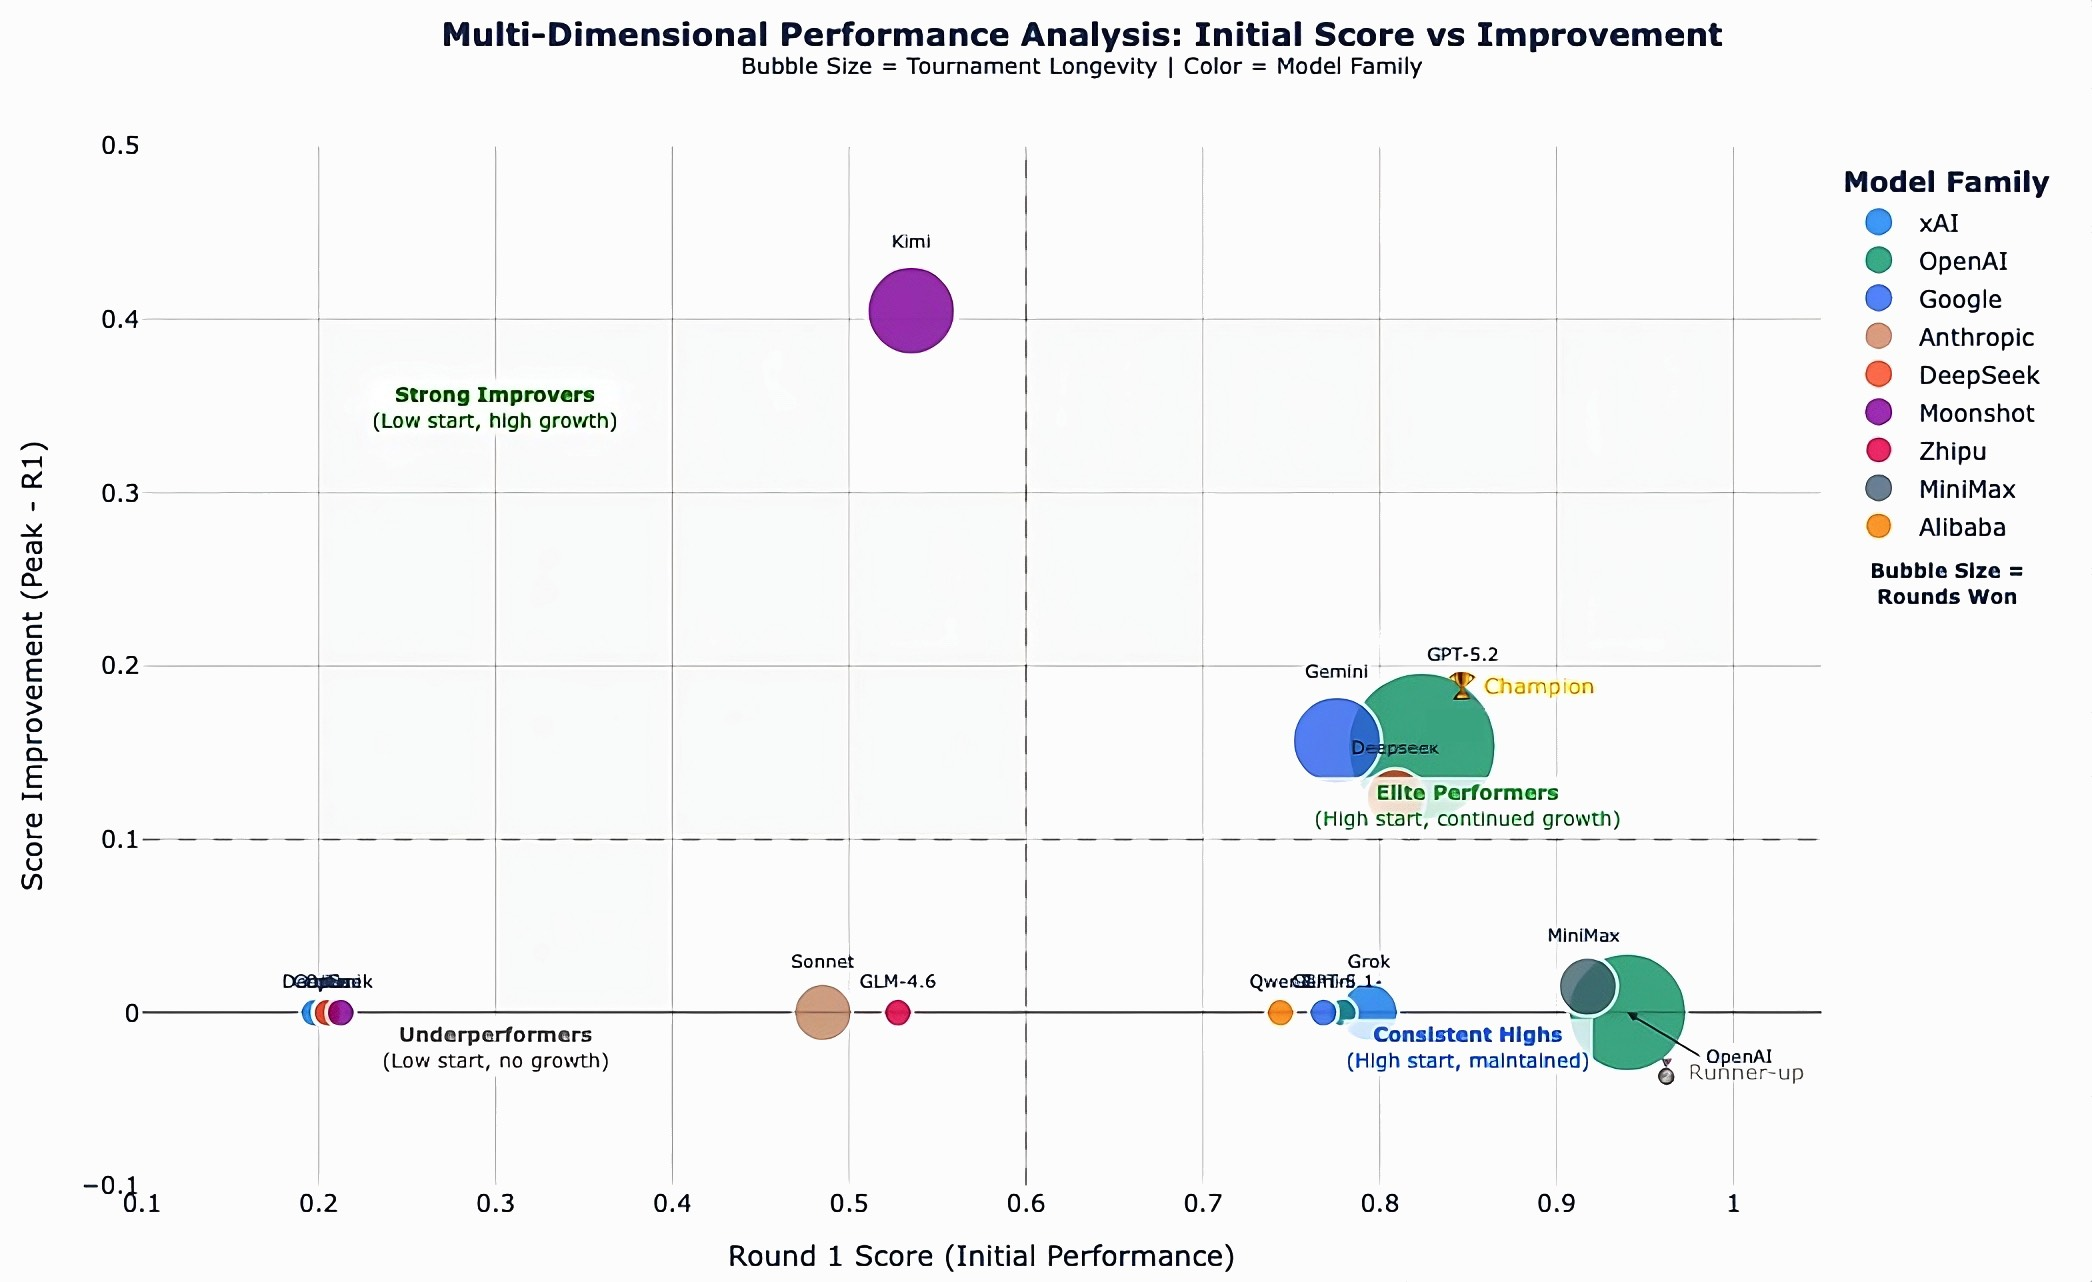
\includegraphics[width=1.0\linewidth, trim={0 0 0 0}, clip]{Images/Improve_Score.jpg}
    % \vspace{0.1cm}
    \caption{Largest Model Improvements After First Round are Highest}
    \label{ScoreImprovementKimi}
\end{figure}

\end{minipage}






\begin{minipage}{\textwidth}




\begin{figure}[H]
    \centering \hspace{-0.2cm}
    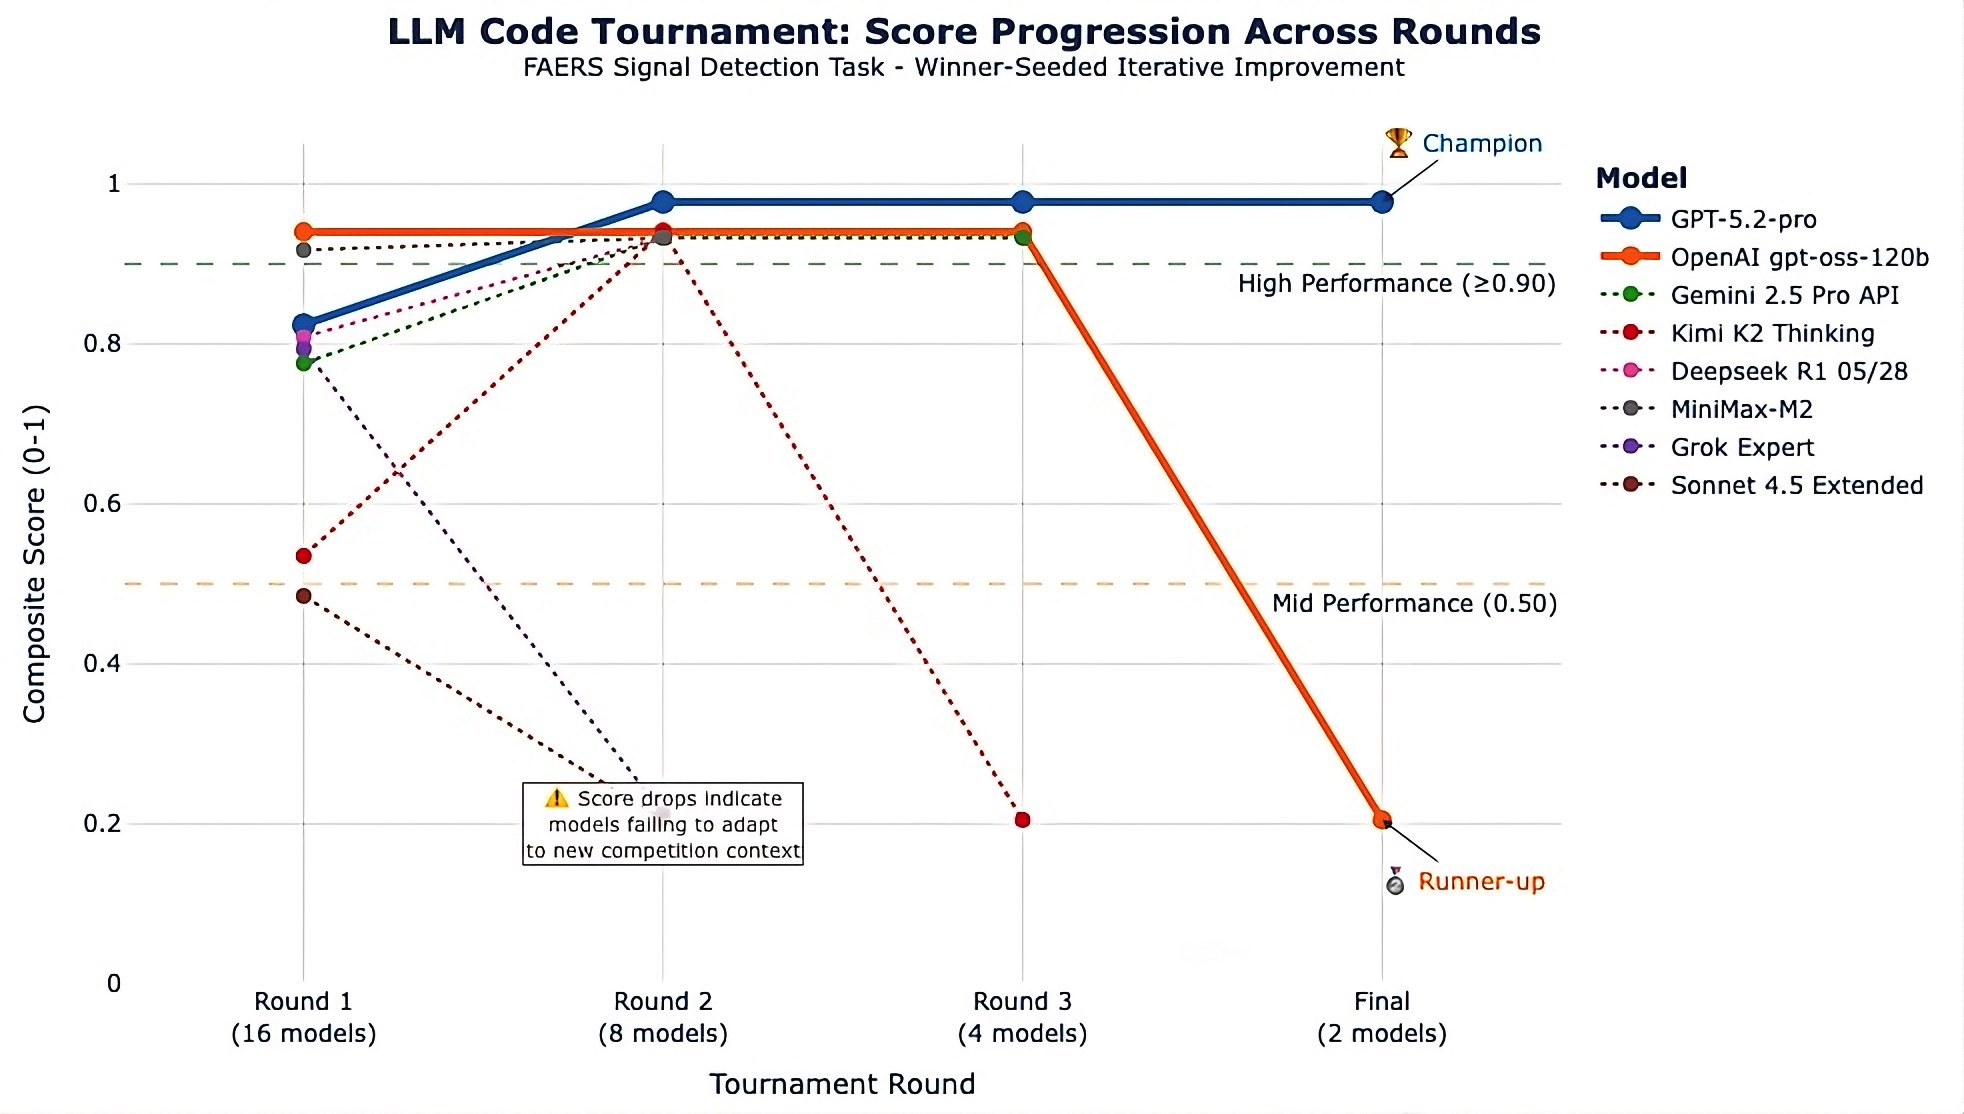
\includegraphics[width=1.01\linewidth, trim={0 0 0 0}, clip]{Images/Score_Progression.jpg}
    % \vspace{0.1cm}
    \caption{Scoring Progression of LLM Code: Inclines Represent Increases}
    \label{ScoreProgressionChampion}
\end{figure} 





\begin{figure}[H]
    \centering
    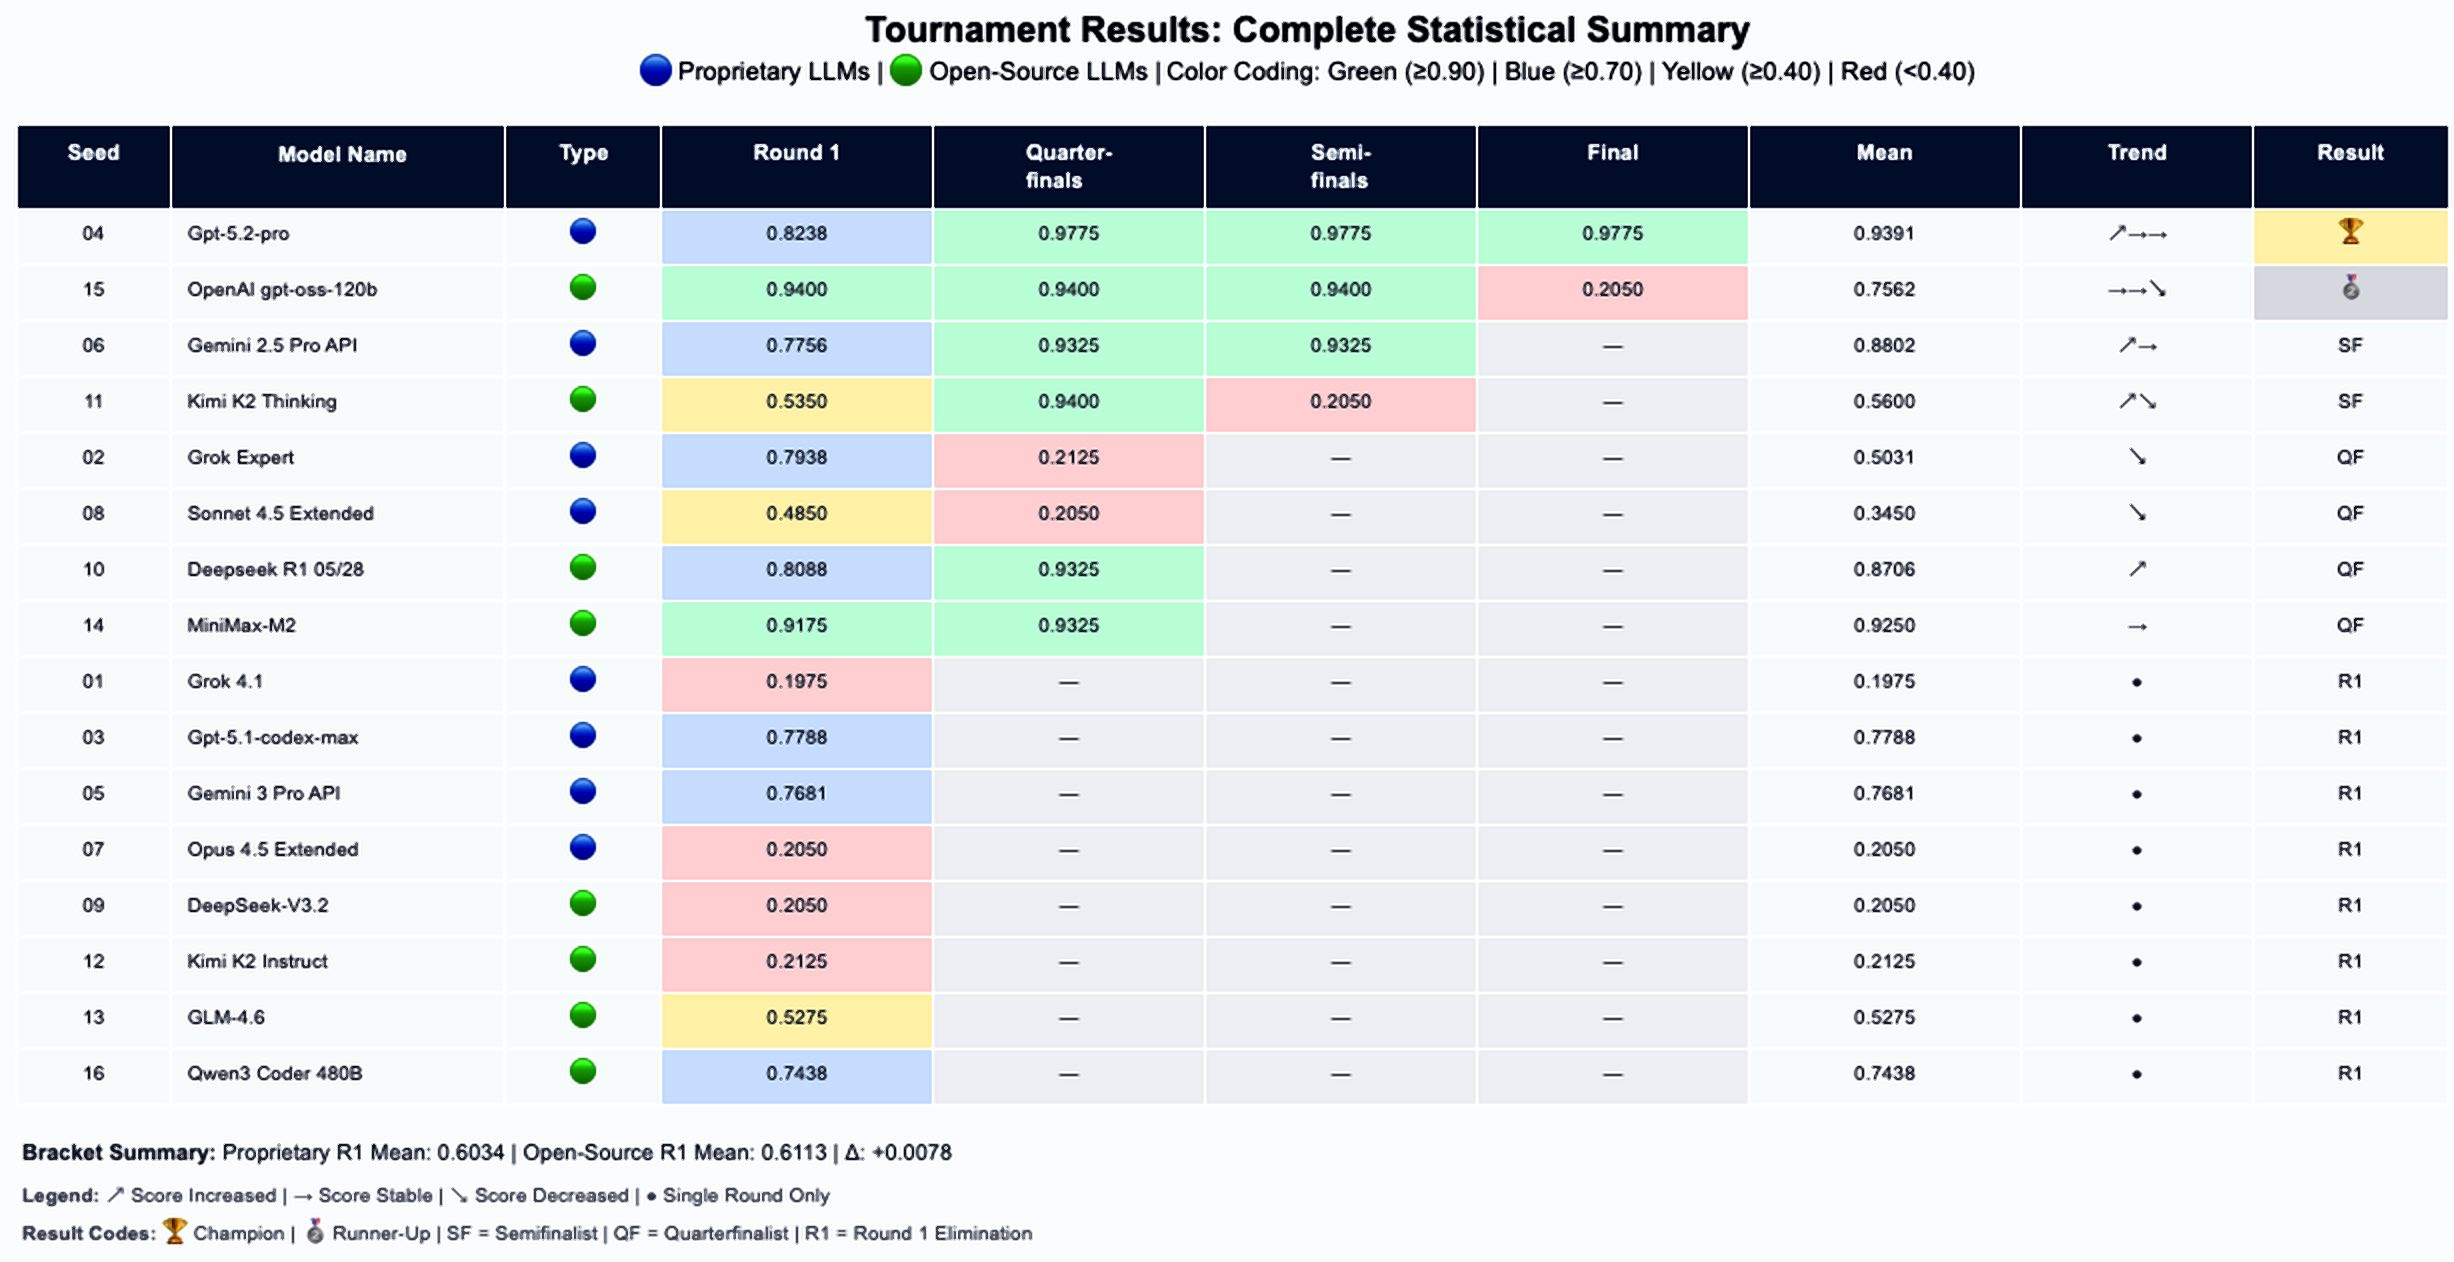
\includegraphics[width=1\linewidth, trim={0 0 0 0}, clip]{Images/Tournament_Results.jpg}
    % \vspace{0.1cm}
    \caption{Statistical Scoring History for All 16 Models Across 4 Rounds}
    \label{ResultsStatisticalHistory}
\end{figure}

\end{minipage}


\begin{minipage}{\textwidth}




\begin{figure}[H]
    \centering
    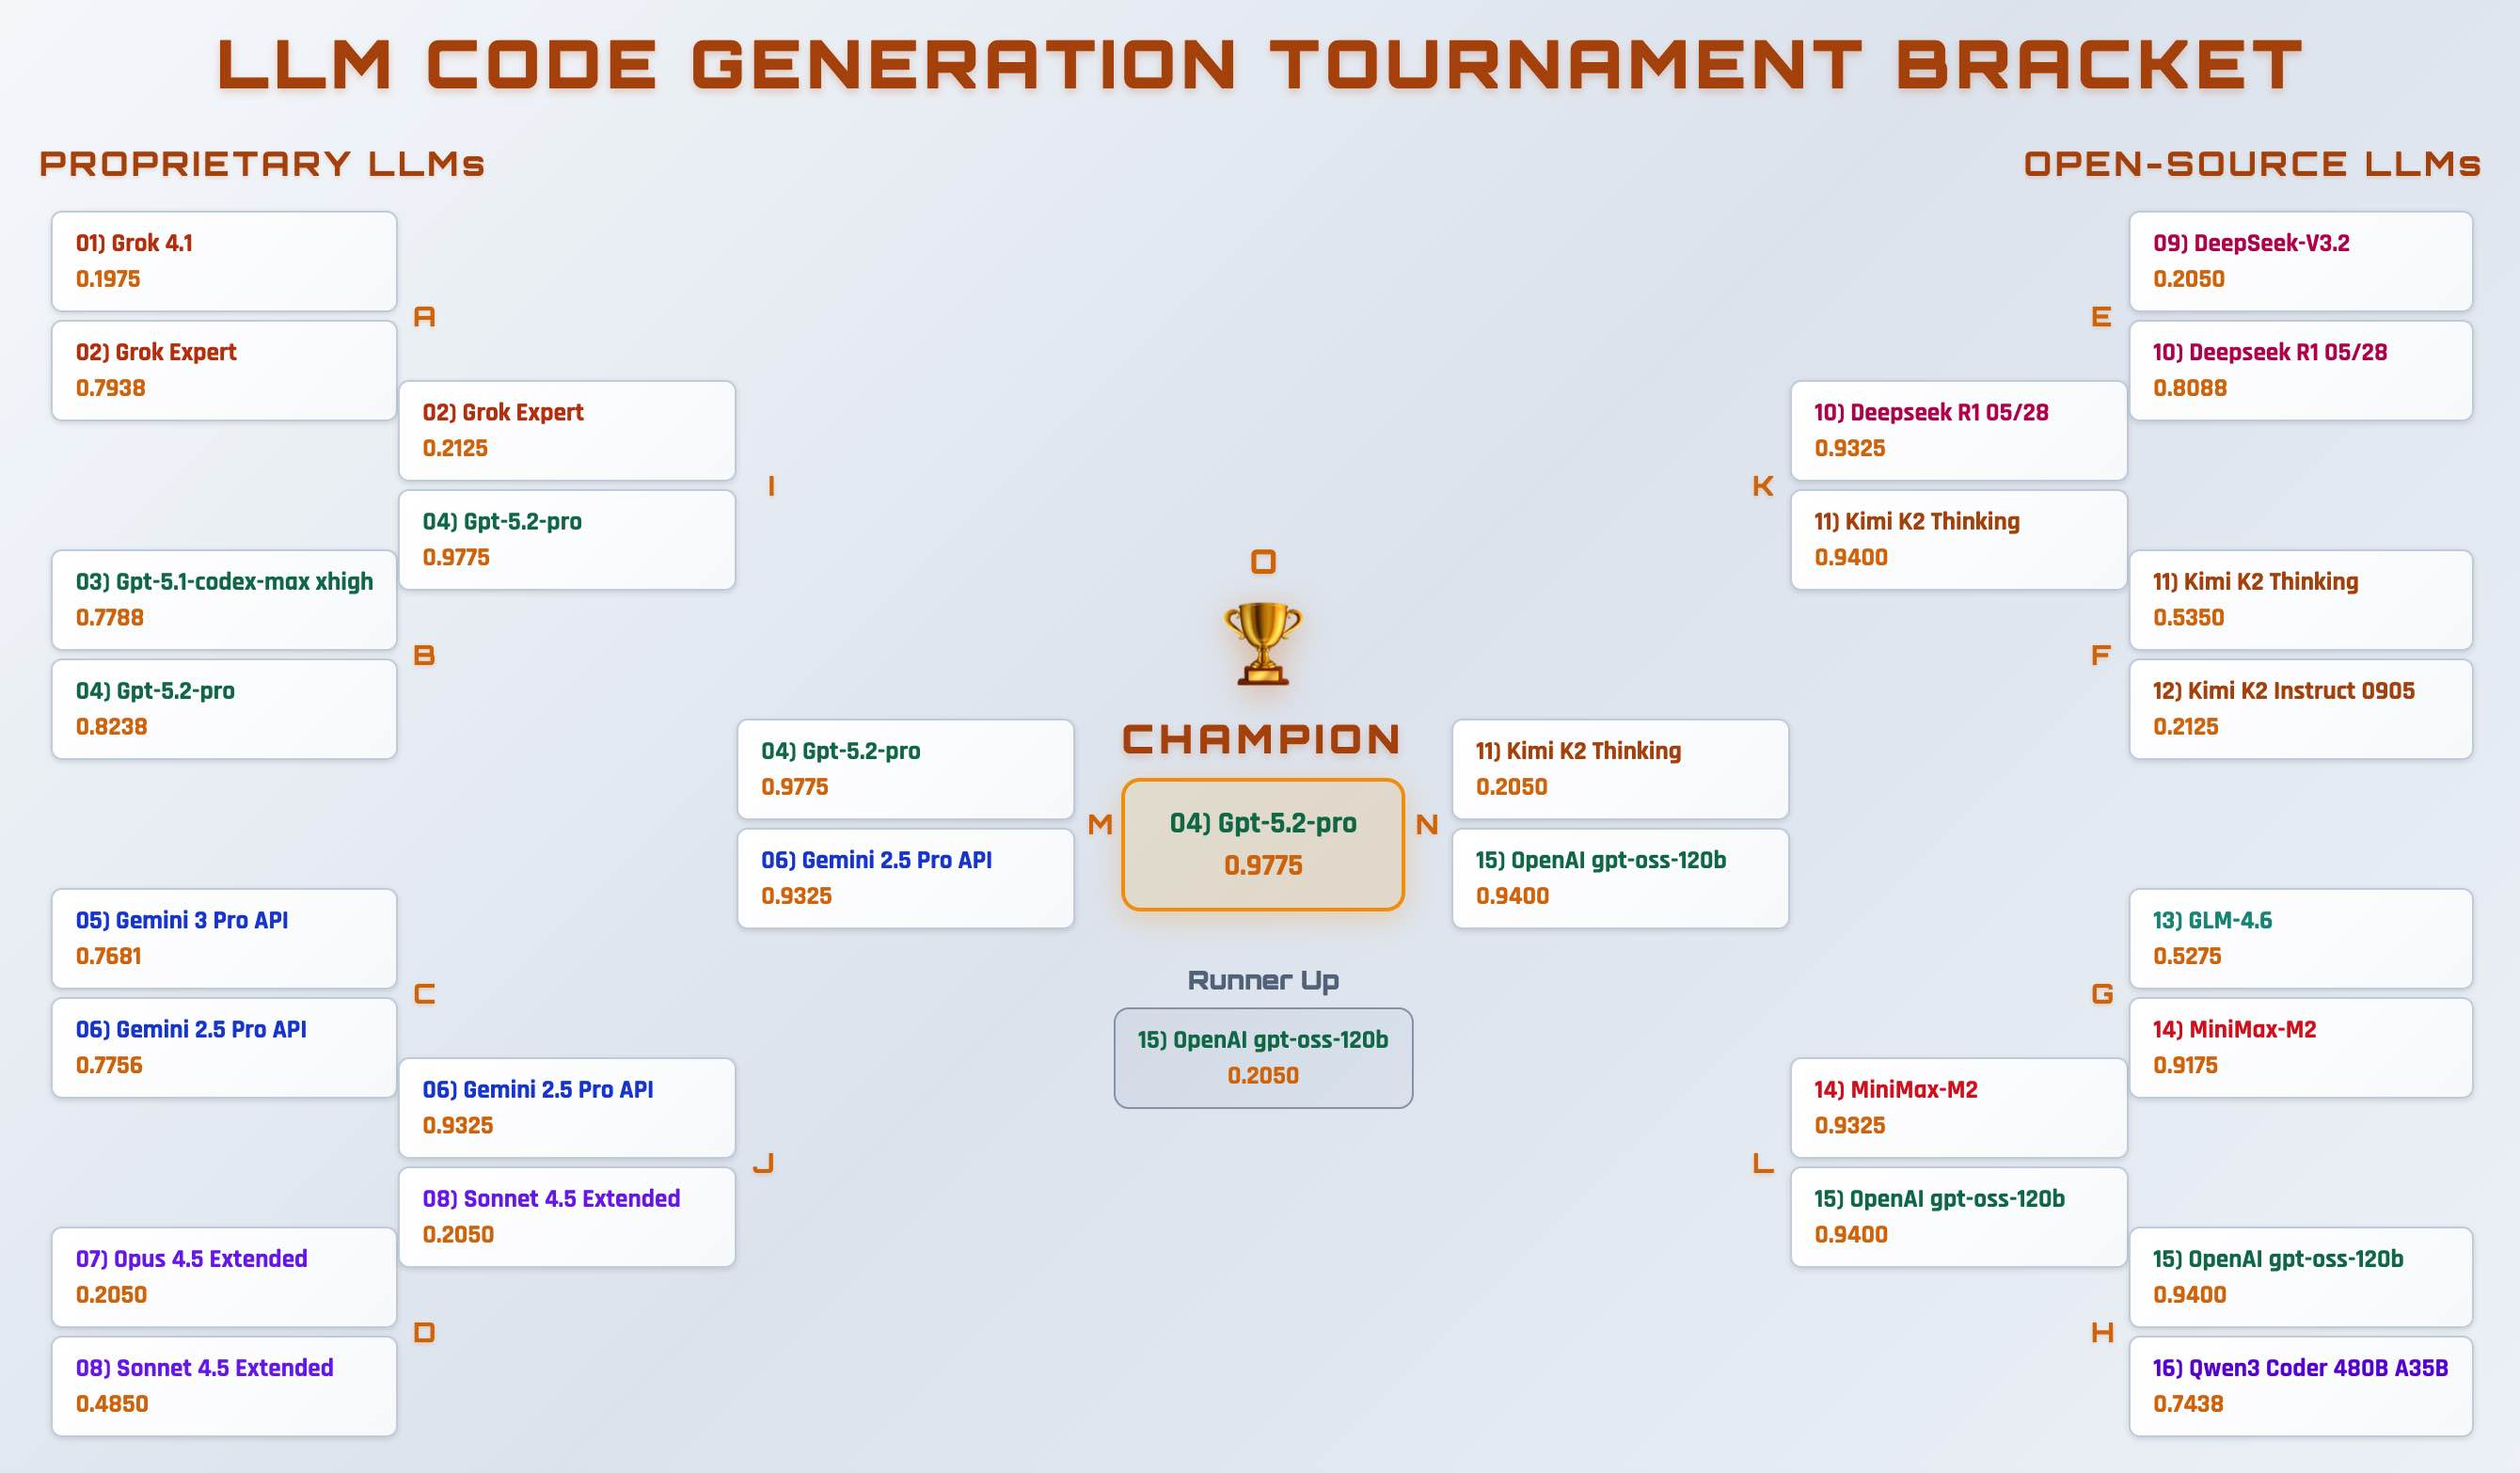
\includegraphics[width=1.0\linewidth, trim={0 0 0 0}, clip]{Images/Bracket_After.jpg}
    % \vspace{0.1cm}
    \caption{Final Championship Results of All 16 LLM Contestants and Scores}
    \label{FinalBracketChampionship}
\end{figure}


\vspace{-0.4cm}

\section{Discussion}

\subsection{Academic Paper References}


 

\newlength{\tablewidthI}
\setlength{\tablewidthI}{17.85cm}

\renewcommand{\arraystretch}{1.45}
\setlength{\tabcolsep}{4pt}

\noindent
\begin{tabular}{|p{0.03\tablewidthI}|p{0.355\tablewidthI}|p{0.15\tablewidthI}|p{0.06\tablewidthI}|p{0.31\tablewidthI}|}
\hline
\multicolumn{5}{|c|}{\rule{0pt}{12pt}\textbf{Academic Paper References for Iterative LLM Code Improvement}\rule[-6pt]{0pt}{6pt}} \\
\hline
\raggedright\textbf{\#} & \raggedright\textbf{Paper Title} & \raggedright\textbf{Authors} & \raggedright\textbf{Year} & \raggedright\arraybackslash\textbf{Relevance to Competition} \\
\hline
\raggedright 1 & \raggedright Self-Refine: Iterative Refinement with Self-Feedback \cite{01BodyMadaan} & \raggedright Madaan et al. & \raggedright 2023 & \raggedright\arraybackslash Core paradigm: Round N notebook $\rightarrow$ Round N+1 code \\
\hline
\raggedright 2 & \raggedright Evaluating Large Language Models Trained on Code \cite{02BodyChen} & \raggedright Chen et al. & \raggedright 2021 & \raggedright\arraybackslash Correctness metric foundation (pass@k) \\
\hline
\raggedright 3 & \raggedright Rethinking the Role of Demonstrations: What Makes In-Context Learning Work? \cite{03BodyMin}& \raggedright Min et al. & \raggedright 2022 & \raggedright\arraybackslash Prior Code\_A/Code\_B as few-shot examples \\
\hline
\raggedright 4 & \raggedright ChatDev: Communicative Agents for Software Development \cite{04BodyQian} & \raggedright Qian et al. & \raggedright 2023 & \raggedright\arraybackslash Multi-agent head-to-head code competition \\
\hline
\raggedright 5 & \raggedright CodeRL: Mastering Code Generation through Deep Reinforcement Learning \cite{05BodyLe} & \raggedright Le et al. & \raggedright 2022 & \raggedright\arraybackslash Execution-based reward (Correctness=45\% weight) \\
\hline
\raggedright 6 & \raggedright CodeClash: Benchmarking Goal-Oriented Software Engineering \cite{03LimitsCodeClash} & \raggedright Yang et al. & \raggedright 2025 & \raggedright\arraybackslash Multi-round tournament to build the best Python function \\
\hline
\end{tabular}

\vspace{-0.1em}
\noindent
{\captionsetup{width=\tablewidthCorr}
\captionof{table}{Academic Papers Relevant to Multi-Round Iterative Learning Process}
\label{AcademicPaperRelevance}

\vspace{0.2cm}

\hspace{1.3em} The current competition builds off of techniques established in prior LLM application papers. For instance, the current study implements Self-Refine (Paper 1) across 4 rounds \cite{01BodyMadaan}, where each model receives its prior round’s notebook as in-context learning demonstrations (Paper 3) \cite{03BodyMin}. Correctness scoring against a Reference Solution parallels CodeRL’s execution feedback (Paper 5) \cite{05BodyLe}. The head-to-head format is akin to ChatDev’s multi-agent collaboration (Paper 4) \cite{04BodyQian}.\ Additionally, the CodeClash goal-based benchmark from the SWE-bench Team regarding LLMs competing in multi-round game tournaments to build the best codebase for achieving a competitive objective was a framework for the study (Paper 6) \cite{03LimitsCodeClash}; where an increased competition pool size from 8 to 16 and a medical objective were additive. The FDA FAERS data files \cite{09BodyFAERS} used in the competition task are known in literature to be effective for providing safety assessments throughout the life cycle of a drug \cite{06BodyPotter}, providing new and unexpected signals of adverse drug reactions \cite{07BodyYang}, and discovering top drugs based on events leading to death \cite{08BodyYu}.


\end{minipage}








\begin{minipage}{\textwidth}

\subsection{Difficulty Benchmarking}

\hspace{1.3em} Answer key creation was easier for the notebook to establish than executing either Code A or Code B due to the solution being fully deterministic with no ambiguity, while competition code must consider many more rows and drug-reaction combinations. Difficulty standards of the \autoref{StandardSWE}-\autoref{StandardCompositeDiff} were calculated by Opus 4.5 Extended.

\vspace{0.1cm}
\hspace{0.8em} \textbf{Reference Solution Code}
\vspace{-0.6cm}\\
\begin{itemize} [leftmargin=2.2em, itemsep=-0.1em, topsep=0.9em]
    \item No programmatic creativity requirements
    \item Already knows how the tables must be merged
    \item Already knows correct logic, date, and quarter parsing rules
\end{itemize}

\vspace{-0.2cm}
\hspace{0.8em} \textbf{Competition Code Must Run}
\vspace{-0.6cm}\\
\begin{itemize} [leftmargin=2.2em, itemsep=-0.1em, topsep=0.95em]
    \item The full sampled FAERS subset, which can be thousands of rows
    \item All combinations of drug × reaction considered, yielding very large numbers
    \item All time-cumulative quarter calculations, which multiplies the number of operations
\end{itemize}




\subsection{Difficulty Benchmarking Standards}

\vspace{0.1cm}

\newlength{\tablewidthA}
\setlength{\tablewidthA}{17.5cm}

\renewcommand{\arraystretch}{1.45}
\setlength{\tabcolsep}{4pt}

\noindent
\begin{tabular}{|p{0.14\tablewidthA}|p{0.22\tablewidthA}|p{0.22\tablewidthA}|p{0.22\tablewidthA}|p{0.14\tablewidthA}|}
\hline 
\multicolumn{5}{|c|}{\rule{0pt}{12pt}\textbf{Software Engineering Complexity Standards}\rule[-6pt]{0pt}{6pt}} \\
\hline
\raggedright\textbf{Standard} & \raggedright\textbf{Metric} & \raggedright\textbf{Task 1 Value} & \raggedright\textbf{Industry Benchmark} & \raggedright\arraybackslash\textbf{Difficulty Rating} \\
\hline
\raggedright McCabe & \raggedright Cyclomatic Complexity & \raggedright 25--35 & \raggedright $>$20 = High Risk & \raggedright\arraybackslash 8.0/10 \\
\hline
\raggedright Halstead & \raggedright Difficulty (D) & \raggedright $\sim$32 & \raggedright $>$30 = Challenging & \raggedright\arraybackslash 7.5/10 \\
\hline
\raggedright Halstead & \raggedright Effort (E) & \raggedright $\sim$90,000 & \raggedright $>$50K = Substantial & \raggedright\arraybackslash 8.0/10 \\
\hline
\raggedright Halstead & \raggedright Time to Program & \raggedright $\sim$83 min & \raggedright $>$60 min = Complex & \raggedright\arraybackslash 7.0/10 \\
\hline
\raggedright COCOMO II & \raggedright Effort & \raggedright 0.6 person-months & \raggedright 0.5--1.0 = Medium & \raggedright\arraybackslash 6.5/10 \\
\hline
\raggedright Lines of Code & \raggedright Implementation Size & \raggedright 150--230 LOC & \raggedright 100--300 = Medium & \raggedright\arraybackslash 6.0/10 \\
\hline
 & & & \raggedright\textbf{Subtotal Average} & \raggedright\arraybackslash\textbf{7.17/10} \\
\hline
\end{tabular}

% \vspace{-0.1em}
\noindent
{\captionsetup{width=\tablewidthCorr}
\captionof{table}{Software Engineering Complexity Assessment Metrics Derived from Static\\Analysis of detect\_signal\_emergence\_improved Function Specification (TASK\_1\_SPEC)}
\label{StandardSWE}




\vspace{0.4cm}

\newlength{\tablewidthB}
\setlength{\tablewidthB}{17.5cm}

\renewcommand{\arraystretch}{1.45}
\setlength{\tabcolsep}{4pt}

\noindent
\begin{tabular}{|p{0.18\tablewidthB}|p{0.28\tablewidthB}|p{0.36\tablewidthB}|p{0.14\tablewidthB}|}
\hline
\multicolumn{4}{|c|}{\rule{0pt}{12pt}\textbf{AI/ML Benchmark Alignment Standards}\rule[-6pt]{0pt}{6pt}} \\
\hline
\raggedright\textbf{Benchmark} & \raggedright\textbf{Criterion} & \raggedright\textbf{Task 1 Mapping} & \raggedright\arraybackslash\textbf{Score (0--10)} \\
\hline
\raggedright HumanEval & \raggedright Function Signature & \raggedright Exact DataFrame params required & \raggedright\arraybackslash 7.0 \\
\hline
\raggedright HumanEval & \raggedright Docstring Comprehension & \raggedright TASK\_1\_SPEC interpretation & \raggedright\arraybackslash 8.0 \\
\hline
\raggedright HumanEval & \raggedright Edge Case Handling & \raggedright Empty inputs, invalid dates, missing cols & \raggedright\arraybackslash 9.0 \\
\hline
\raggedright HumanEval & \raggedright Algorithmic Correctness & \raggedright PRR formula + temporal emergence & \raggedright\arraybackslash 9.0 \\
\hline
\raggedright HumanEval & \raggedright Output Validation & \raggedright 6-column schema compliance & \raggedright\arraybackslash 6.0 \\
\hline
\raggedright MBPP & \raggedright Problem Category & \raggedright Level 4--5 (Advanced/Expert) & \raggedright\arraybackslash 8.5 \\
\hline
\raggedright BigCodeBench & \raggedright Tier Classification & \raggedright Tier 3--4 (Domain + Multi-source) & \raggedright\arraybackslash 8.0 \\
\hline
\raggedright APPS & \raggedright Difficulty Band & \raggedright Interview-level (comparable) & \raggedright\arraybackslash 7.5 \\
\hline
 & & \raggedright\textbf{Subtotal Average} & \raggedright\arraybackslash\textbf{7.88/10} \\
\hline
\end{tabular}

% \vspace{0.1em}
\noindent
{\captionsetup{width=\tablewidthCorr}
\captionof{table}{Established AI/ML Code Generation Benchmarks. Edge Case Handling Scored Highest (9.0)}
\label{StandardAIML}
\end{minipage}





\begin{minipage}{\textwidth}


\vspace{0.4cm}


\newlength{\tablewidthC}
\setlength{\tablewidthC}{17.5cm}

\renewcommand{\arraystretch}{1.45}
\setlength{\tabcolsep}{4pt}

\noindent
\begin{tabular}{|p{0.18\tablewidthC}|p{0.28\tablewidthC}|p{0.36\tablewidthC}|p{0.14\tablewidthC}|}
\hline
\multicolumn{4}{|c|}{\rule{0pt}{12pt}\textbf{FDA/Pharmacovigilance Regulatory Standards}\rule[-6pt]{0pt}{6pt}} \\
\hline
\raggedright\textbf{Standard} & \raggedright\textbf{Component} & \raggedright\textbf{Implementation Requirement} & \raggedright\arraybackslash\textbf{Complexity Multiplier} \\
\hline
\raggedright ICH E2B(R3) & \raggedright Case Identification & \raggedright primaryid linkage (3 tables) & \raggedright\arraybackslash 1.5$\times$ \\
\hline
\raggedright ICH E2B(R3) & \raggedright Drug Characterization & \raggedright role\_cod suspect filtering & \raggedright\arraybackslash 1.2$\times$ \\
\hline
\raggedright ICH E2B(R3) & \raggedright Reaction Coding & \raggedright MedDRA PT handling & \raggedright\arraybackslash 1.1$\times$ \\
\hline
\raggedright ICH E2B(R3) & \raggedright Temporal Analysis & \raggedright event\_dt $\rightarrow$ quarter conversion & \raggedright\arraybackslash 1.8$\times$ \\
\hline
\raggedright CIOMS VI & \raggedright Signal Detection & \raggedright PRR $\geq$ 2.0, N $\geq$ 3 threshold & \raggedright\arraybackslash 1.3$\times$ \\
\hline
\raggedright EMA Guidelines & \raggedright Disproportionality & \raggedright Expected vs.\ observed ratio & \raggedright\arraybackslash 1.4$\times$ \\
\hline
 & & \raggedright\textbf{Cumulative Complexity Factor} & \raggedright\arraybackslash\textbf{2.97$\times$} \\
\hline
 
\raggedright Base Difficulty & \raggedright 5.0 (standard data task) & \raggedright \textbf{5.0} & \raggedright\arraybackslash — \\
\hline
\raggedright Adjusted Difficulty & \raggedright 5.0 $\times$ 2.97 $\div$ 2 & \raggedright \textbf{Derived Difficulty Score} & \raggedright\arraybackslash\textbf{7.43/10} \\
\hline
\end{tabular}

\vspace{-0.1em}
\noindent
{\captionsetup{width=\tablewidthCorr}
\captionof{table}{FDA Complexity: Expected = (drug\_cases * reac\_cases) / total\_cases; prr = pair\_cases / expected}
\label{StandardFDAPharmac}




\vspace{0.4cm}


\newlength{\tablewidthD}
\setlength{\tablewidthD}{18.05cm}

\renewcommand{\arraystretch}{1.45}
\setlength{\tabcolsep}{4pt}

\noindent
\begin{tabular}{|p{0.22\tablewidthD}|p{0.38\tablewidthD}|p{0.18\tablewidthD}|p{0.14\tablewidthD}|}
\hline
\multicolumn{4}{|c|}{\rule{0pt}{12pt}\textbf{Data Complexity Assessment (FAERS-Specific)}\rule[-6pt]{0pt}{6pt}} \\
\hline
\raggedright\textbf{Data Characteristic} & \raggedright\textbf{Description} & \raggedright\textbf{Challenge Level} & \raggedright\arraybackslash\textbf{Score (0--10)} \\
\hline
\raggedright Relational Structure & \raggedright 3-table inner joins required & \raggedright High & \raggedright\arraybackslash 8.0 \\
\hline
\raggedright Date Format Variability & \raggedright YYYYMMDD, YYYYMM, decimal suffixes & \raggedright High & \raggedright\arraybackslash 8.5 \\
\hline
\raggedright Missing Data Prevalence & \raggedright Requires dropna/fillna handling & \raggedright Moderate & \raggedright\arraybackslash 6.5 \\
\hline
\raggedright Case Deduplication & \raggedright nunique() on primaryid & \raggedright Moderate & \raggedright\arraybackslash 6.0 \\
\hline
\raggedright Volume Scalability & \raggedright 400K+ records (full dataset) & \raggedright High & \raggedright\arraybackslash 7.5 \\
\hline
\raggedright Schema Variability & \raggedright Column casing, whitespace & \raggedright Moderate & \raggedright\arraybackslash 6.5 \\
\hline
\raggedright Temporal Granularity & \raggedright Quarterly aggregation logic & \raggedright High & \raggedright\arraybackslash 8.0 \\
\hline
 & & \raggedright\textbf{Subtotal Average} & \raggedright\arraybackslash\textbf{7.29/10} \\
\hline
\end{tabular}

\vspace{-0.1em}
\noindent
{\captionsetup{width=\tablewidthCorr}
\captionof{table}{FAERS Dataset Complexity: Schema Variability (6.5) Applied via columns.str.lower().str.strip()}
\label{StandardDataComplex}






\vspace{0.4cm}

\newlength{\tablewidthE}
\setlength{\tablewidthE}{17.8cm}

\renewcommand{\arraystretch}{1.45}
\setlength{\tabcolsep}{4pt}

\noindent
\begin{tabular}{|p{0.26\tablewidthE}|p{0.22\tablewidthE}|p{0.14\tablewidthE}|p{0.14\tablewidthE}|p{0.16\tablewidthE}|}
\hline
\multicolumn{5}{|c|}{\rule{0pt}{12pt}\textbf{Composite Difficulty Score Calculation}\rule[-6pt]{0pt}{6pt}} \\
\hline
\raggedright\textbf{Dimension} & \raggedright\textbf{Source Table} & \raggedright\textbf{Score} & \raggedright\textbf{Weight} & \raggedright\arraybackslash\textbf{Weighted Score} \\
\hline
\raggedright Software Engineering & \raggedright Table A & \raggedright 7.17 & \raggedright 20\% & \raggedright\arraybackslash 1.434 \\
\hline
\raggedright AI/ML Benchmarks & \raggedright Table B & \raggedright 7.88 & \raggedright 25\% & \raggedright\arraybackslash 1.970 \\
\hline
\raggedright Regulatory Standards & \raggedright Table C & \raggedright 7.43 & \raggedright 25\% & \raggedright\arraybackslash 1.858 \\
\hline
\raggedright Data Complexity & \raggedright Table D & \raggedright 7.29 & \raggedright 20\% & \raggedright\arraybackslash 1.458 \\
\hline
\raggedright Domain Expertise Required & \raggedright (Expert estimate) & \raggedright 8.50 & \raggedright 10\% & \raggedright\arraybackslash 0.850 \\
\hline
\raggedright\textbf{TOTAL} & & & \raggedright\textbf{100\%} & \raggedright\arraybackslash\textbf{7.57/10} \\
\hline
\end{tabular}

\vspace{-0.1em}
\noindent
{\captionsetup{width=\tablewidthCorr}
\captionof{table}{Weighted Composite Difficulty Score Representing Task-Level Complexity Across 4 Tournament Rounds}
\label{StandardCompositeDiff}
\end{minipage}
 


\begin{minipage}{\textwidth} 

 
\vspace{-0.4cm}






\section{Limitations and Future Work}

\hspace{1.3em} All LLMs run in the study were either on \$20 OpenAI, \$20 Anthropic, \$30 xAI monthly plans, or using pay per token API playgrounds: Gpt \$7.47, Open-source \$0.59; \$78.06 Total. A limitation was in accessing additional high tier models including Google AI Ultra's "Deep Think" feature "which uses parallel processing to evaluate multiple options and refine answers quickly. This results in fewer errors in complex tasks like advanced math, scientific modeling, and high-stakes financial projections". This option was cost prohibitive for the study at a standard price of \$249.99/month \cite{01LimitsGemUltra}. Similarly, xAI's SuperGrok Heavy is meant "for professionals performing heavy reasoning, automation workflows, dense analytical tasks, coding support, multi-step problem solving" \cite{02LimitsGrokHeavy}, but costs \$300/month. In either of these two model tiers, the manufacturer's current models likely evaluate multiple generations based on the same prompt to increase the likelihood of returning a single best answer. 

\vspace{0.2cm} 

\hspace{1.3em} Another limitation was in the development of the Round 0 notebook used by all 16 models to generate their first code submission that was run in the Round 1 competition notebook. The Round 0 notebook was based on lower score initial competitors (0.8750/0.8875) which may have limited Round 1 score performance. Similarly, the Round 0 notebook used to generate Round 1 code was based on a different correctness metric regarding a reference standard, which may have also caused lower than expected Round 1 scores. Regardless, the goal provided to both Round 1 and Round 2-4 contestants remained the same "to achieve a perfect score of 1.0" despite minor notebook differences. Attempts to increase FAERS Dataset incorporation beyond the tournament's "0.1" sample fraction setting were not successful, as shown in Prompt\_10. The notebook development process did occur a truncation in the number of notebook outputs from the Round 0 to Round 1, as the competition task became better defined. This main effect was that the AI peer review process instructions originally outputted inside the notebook containing competition functions, scores, and additional insights became reduced, and were relocated as file outputs. 

\vspace{0.2cm} 

\hspace{1.3em} To accommodate for the truncation, code generations for Rounds 2-4 were provided the "Instructions for Improvement" section from Round 0 to assist LLMs in the competition task, and the exact function response format. Based on the CodeClash paper's findings \cite{03LimitsCodeClash} regarding limitations of processing end-of-match log files, a similar approach was taken in the current study by solely focusing on the processing of a match winner's previously completed notebook. Suitable information existed regarding both competitor's code, code results, and other adjustments based on the notebook's format and system to make informed code changes. The additional +100 line "08\_competition\_report.json" would likely overwhelm LLMs and cause poor final scores, based on the author's best prior results limiting the number of inputs for working and high performance code \cite{21KawchakPaper, 20KawchakPaper, 19KawchakPaper}. Another limitation was observed in high correctness and methodology score penalties for unexecutable competition code (-0.7500), as there were 7 scores at 0.2125 or below. Future studies will focus on oncology LLM-generated code at scale.




\section{Conclusions}

\hspace{1.3em} Human code iterations have increased efficiency with the aid of interactive debugging and profiling tools. However, manual optimization, time-consuming, and labor-intensive limitations have led to worker fatigue and diminishing returns. AI code iterations have automated the use of algorithms with the use of search-based optimization, genetic programming, automated program repair, reinforcement learning, and ML-guided compilers.\ This includes DeepMind's 2022 AlphaTensor \cite{10IntroAlphaTensor} and 2023 AlphaDev \cite{09IntroAlphaDev} projects that used reinforcement learning to discover new matrix multiplication algorithms and algorithm discovery being treated as a game. However, these type of pre-LLM coding iterations were typically rigid - in that code must be machine-readable, with the improvement goal encoded as a fitness function or reward. Fast forward to late 2025, and LLMs now consistently provide an enhanced number of utilities to quickly iterate code and utilize natural language interactions with humans across full R\&D areas. 

\vspace{0.2cm} 

\hspace{1.3em} The 2025 DeepMind AlphaEvolve \cite{21IntroAlphaEvolve} now uses algorithmic AI agents combining evolutionary search with LLM-guided code generation to iteratively evolve algorithms. Several academic papers have laid the groundwork regarding iterative refinement \cite{01BodyMadaan}, LLM evaluation \cite{02BodyChen}, in-context learning \cite{03BodyMin}, chat-based coding competitions \cite{04BodyQian}, and reward-based code generation \cite{05BodyLe}. The November 2025 CodeClash LLM-generated code competition by Yang et al. \cite{03LimitsCodeClash} provided a compelling 8 contestant multi-game format in which Claude Sonnet 4.5 took the highest overall score. Since the results were published, November/December 2025 industry additions of Grok 4.1, Gpt-5.2-pro, Gemini 3 Pro, Opus 4.5, and DeepSeek-V3.2 were found to warrant a larger 16 contestant pool based on the pharmaceutical industry relevant FDA Adverse Event Reporting System (FAERS) latest quarterly data files (25Q3). The 8 proprietary vs.\ 8 open-source LLM single-elimination code generation tournament was based on a Python competition notebook developed by Opus 4.5 Extended. A total of 12 software engineering prompts were utilized in order to 1) Optimize the FAERS four signal reference-solution output based on the "First calendar quarters where pair becomes a safety “signal” (PRR \raisebox{0.25ex}{\scalebox{0.7}{$\geq$}} threshold AND count \raisebox{0.25ex}{\scalebox{0.7}{$\geq$}} minimum cases)", 2) Fix errors, and 3) Develop the prompt instructing LLMs to generate competition code. 

\vspace{0.2cm} 

\hspace{1.3em} First Round winners saw upsets between proprietary LLM manufacturer pairs of Gemini 2.5 Pro API (0.7756) defeating Gemini 3 Pro API (0.7681); as well as open-source LLM manufacturer pairs of DeepSeek R1 05/28 (0.8088) defeating DeepSeek-V3.2 (0.2050). The surprising first round best score was achieved by OpenAl gpt-oss-120b at 0.9400. To generate subsequent rounds of competition code, each winning LLM was provided with the competition prompt and their prior notebook based on competitors' code, match code, and match results to iteratively learn and generate new code. Round 1-2 iterative learning scores increased for 4/8 of the contestants, most notably with Kimi K2 Thinking having the largest single round increase of the tournament from 0.5350 to 0.9400 (+0.405). From Round 2 to Round 3, 3/4 teams maintained their previous round's score with semifinal proprietary LLM scores featuring a Gpt-5.2-pro (0.9775) victory over Gemini 2.5 Pro API (0.9325). Open-source LLM scores of OpenAl gpt-oss-120b (0.9400) overcame Kimi K2 Thinking (0.2050). Championship results featured Gpt-5.2-pro maintaining its 0.9775 score victory over OpenAl gpt-oss-120b (0.2050); marking gpt-oss-120b's only non 0.9400 score. Thus, Gpt-5.2-pro emerged as an iterative learner with consistent scores and this Championship tournament winner.

\end{minipage}
 


 




\begin{minipage}{\textwidth}
 
\vspace{-0.2cm}
\section{Prompts}
 
\vspace{-0.5cm}
\renewcommand{\arraystretch}{1.61} % Adjust row height for better readability
\setlength{\tabcolsep}{0pt} % Reduces horizontal padding inside table cells
\begin{table}[H]
\centering
\begin{tabular}{p{17.8cm}}
\toprule
\centering
\vspace{-0.6cm}
\textbf{Prompts 01-06: Notebook Generation} \\
\vspace{0.055cm}
\midrule 
\raggedright \fontsize{9.3pt}{10.3pt}\selectfont
\textbf{Prompt\_01: Initial Python FAERS Competition Notebook.}\\  
Prompt for Generating a Python Notebook: Head-to-Head LLM Code Competition Using FDA FAERS Pharmacovigilance Data\\ 
Purpose and Context\\
Generate a Python notebook designed for execution on a Google Colab T4 GPU environment that implements a structured head-to-head competition framework for evaluating LLM-generated code. The competition uses real-world pharmacovigilance data from the FDA Adverse Event Reporting System (FAERS) Q3 2025 Quarterly Data Extract.
\mbox{[See Supplementary Notebook\_Generation for Full Prompt]}
\midrule 
\raggedright \fontsize{9.3pt}{10.3pt}\selectfont
\textbf{Prompt\_02: Improvements: Drive, Sections, ASCII Dataset Samples.} Focus your resources on improving the ipynb. Make sure google drive is incorporated in order to upload the 7 txt file datasets, and also download the full results to specific directories (no data generation is required). Separate cells by section for the Python notebook appropriately. Include instructions for relevant sections that are adjustable. A sample of the dataset files is included for reference: ASCII Dataset Samples.txt. It is important for the competition to surround around the full dataset files (not included due to size). Remove the FDA link, and include this instead: FDA Adverse Event Reporting System (FAERS): Latest Quarterly Data Files. Remove the few shot learning feature inside the competition (only the LLMs' code will run head to head). Be sure to more clearly detail how exactly each LLM’s code is incorporated.
\mbox{[ASCII Dataset Samples.txt]} \\ 
\midrule  
\raggedright \fontsize{9.3pt}{10.3pt}\selectfont
\textbf{Prompt\_03a: ChatGPT Competition Task A, B, C Selection.} For the original attached notebook: Describe which and how the 4 tasks were run for Code A and Code B (were each of the tasks run for both sets of code?). Provide 3 other more constructive and challenging tasks based on the 7 file FAERS dataset in the competition (that no other researchers have likely done before on this dataset)? Right now correctness is 100\%, as this is likely for more trivial tasks. The other issue between Code A and Code B is that the runtimes are not consistent across multiple experiments based on the hardware (and hence the efficiency scores vary). What would be some ways to address this? Or should this issue resolve with more challenging and longer tasks? The overall scores for Code A and B should be consistent for each run and not be thrown off by fluctuating runtimes. 
\mbox{[USER\_FAERS\_LLM\_Competition.ipynb]} \\
\midrule 
\raggedright \fontsize{9.3pt}{10.3pt}\selectfont
\textbf{Prompt\_03b: ChatGPT Competition Additional Task Selection.} No. Similar format and length the originals. Like: �� Task C — Treatment Pathway Reconstruction From THER + INDI + OUTC Objective: Identify the sequence of drug therapies for a given indication and determine outcome likelihood based on therapy order. Requires: * Merge THER with DRUG and INDI * Reconstruct drug start/end dates per case * Infer therapy sequences * Model outcomes by treatment order (e.g., Drug A → Drug B vs. Drug B → Drug A) Novelty: * FAERS is not commonly used for pathway inference due to date quality * This becomes a deep reasoning task for LLMs Hard for LLMs: * Cleaning inconsistent dates * Sorting sequences * Joining three files with time logic * Aggregating outcome patterns
\mbox{[USER\_FAERS\_LLM\_Competition.ipynb]} \\
\midrule 
\raggedright \fontsize{9.3pt}{10.3pt}\selectfont
\textbf{Prompt\_03: Incorporation of Increased Competition Tasks Difficulty.} Your goal is to focus only on updating the provided notebook with the attached more relevant competition tasks that are more challenging and will allow for larger differences in the “Correctness” metrics. The results must be reproducible every time the notebook is run, therefore the “Efficiency” metric should be modified from runtimes to an algorithmic complexity proxy, or other suitable method to approximate runtime. Code\_A score and Code\_B score must not change every time the notebook is re-run. Include runtimes, but not for the use of scoring. New Code\_A and Code\_B code simulating LLM-generated code must be included to address the four included replacement competition tasks. Keep the function all sections of the attached notebook. Return a single new Python notebook. “START NEW COMPETITION TASKS” \mbox{[See Supplementary for Full Tasks]} \\
\midrule 
\raggedright \fontsize{9.3pt}{10.3pt}\selectfont
\textbf{Prompt\_04a: ChatGPT Task A FDA Relevancy Identification.} Based on this notebook. Which competition task is most relevant to FDA, and why? Detail in full. \mbox{[USER\_3rd\_FAERS\_LLM\_Competition.ipynb]}\\
\midrule 
\raggedright \fontsize{9.3pt}{10.3pt}\selectfont
\textbf{Prompt\_04: Error Fixes, Single Competition Task A Identification.} Your goal is to focus only on providing a new Python notebook that fixes the attached notebook errors, and focuses only on the single "Task A: Cross-Table Temporal Signal Emergence Detection" competition task. Therefore there should only be one set of Code A and Code B competition code. Keep the function of all sections of the attached notebook. Return a single new Python notebook.  
\mbox{[USER\_3rd\_FAERS\_LLM\_Competition.ipynb]}\\
\midrule 
\raggedright \fontsize{9.3pt}{10.3pt}\selectfont
\textbf{Prompt\_05: Several Optimizations, Task A to Task 1 Rename.} Produce one optimized Python notebook. Task A should be renamed Task 1. Additionally, all subsequent rounds will aim to improve on the same Task 1. The competition task code needs to be explicitly commented (it should be clear to the user how the task code functions, and where all it is incorporated into the notebook). If one or both of the competition Code do not run, the notebook should finish and state the results appropriately. In the Round Results output: “Algorithmic Efficiency” should be renamed “Algorithmic Effic.” The Peer Review Process cell output needs to include results and code for both Code A and B in the same output. This Peer Review Process output will be provided to both the winner and loser of the competition. The Peer Review Process output should include all necessary instructions, so either LLM can make corrections based on the single Peer Review Process output. The instructions should specify LLMs to output their replacement Python functions in Python, not JSON. Keep the function of all sections of the attached notebook. Return a single new Python notebook.  
\mbox{[USER\_4th\_FAERS\_LLM\_Competition\_TaskA\_Fixed.ipynb]}\\
\midrule 
\raggedright \fontsize{9.3pt}{10.3pt}\selectfont
\textbf{Prompt\_06: Temporal-Signal Task Defined Outside Competition Code.} It appears that the the temporal-signal task is implemented exclusively in the two LLM-generated functions. Should the task be defined in the notebook outside of the competition code? Will future rounds of code be deriving the task from the Code and not explicitly defined in the notebook? Is it possible to have the task defined separately in it's own cell?   
\\

\midrule 
\raggedright
\vspace{-0.35cm}
% Begin Process
\begin{figure}[H]
\begin{center}
\tikzstyle{process} = [rectangle, minimum width=2.5cm, minimum height=1.4cm, text centered, draw=black]
\tikzstyle{arrow} = [line width=1.05pt,->,>=stealth]
\begin{tikzpicture}[node distance=3.075cm]
\node (P1) [process, fill=gray!10, align=center] {First Notebook\\Generation};
\node (P2) [process, fill=gray!17, right of=P1, align=center] {Notebook\\Improvements};
\node (P3) [process, fill=gray!24, right of=P2, align=center] {Competition\\ID Selection};
\node (P4) [process, fill=gray!31, right of=P3, align=center] {Notebook Task\\Implementation};
\node (P5) [process, fill=gray!38, right of=P4, align=center] {Notebook\\Optimizations};
\node (P6) [process, fill=gray!45, right of=P5, align=center] {Signal Task\\Inquiries}; 
\draw [arrow] (P1) -- (P2);
\draw [arrow] (P2) -- (P3);
\draw [arrow] (P3) -- (P4);
\draw [arrow] (P4) -- (P5);
\draw [arrow] (P5) -- (P6); 
\end{tikzpicture}
\end{center}
\end{figure}
% End Process
\vspace{-0.5cm}
\bottomrule 
\end{tabular}
\vspace{0.3cm}
{\captionsetup{width=\tablewidthCorr}
\caption{Opus 4.5 Extended and ChatGPT, Brackets are Attachments. See Supplementary for Prompts, Thoughts, and Outputs}
\label{PromptsTab1}
\end{table}
\end{minipage}







 






\begin{minipage}{\textwidth}

\vspace{-0.75cm}
\renewcommand{\arraystretch}{1.61}  
\setlength{\tabcolsep}{0pt}  
\begin{table}[H]
\centering
\begin{tabular}{p{17.8cm}}
\toprule
\centering
\vspace{-0.6cm}
\textbf{Prompts 07-12: LLM Code Gen \& Notebook Generation} \\
\vspace{0.055cm}
\midrule 
\raggedright \fontsize{9.3pt}{10.3pt}\selectfont
\textbf{Prompt\_07: Meta Prompt for Single New Code Competition Generation.} Design a prompt that will be provided to a LLM that takes in a notebook such as that which is attached, and outputs a single new Code to compete in future notebook competitions (don’t specify Code A or Code B; the generated code could be used for either case). It is important that your prompt directs the LLM to generate new competition code that is based on the notebook, and sections such as the PEER REVIEW PROMPT output. Essentially, the future LLM should be able to make informed decisions from the notebook to achieve a final score of “1.0” based on Correctness, Methodology, Code Quality, and Algorithmic Efficiency. Inform the LLM that it can execute code on its own if that is believed to improve the final score of the Code in the competition. Also instruct the LLM to specify which aspects of notebook sections were used in its decision making process to obtain its new CODE.  
\mbox{[USER\_6th\_FAERS\_LLM\_Competition\_Task1\_v2.ipynb]} \\
\midrule 
\raggedright \fontsize{9.3pt}{10.3pt}\selectfont
\textbf{Prompt\_08: New Notebook Outputs Exact Competition Task in Drive.} Based on the attached notebook, return a new Python notebook that outputs in Drive the exact answer that was used for the task competition, and each of Code A and Code B answers that correspond to the exact solution to allow for head to head comparisons. Currently, there are three output files that don't appear to address these concerns (other similar information needed for a publication should also be outputted, such as (concise and general explanations regarding how the competition task solution and Code A and Code B answers were formed independent on Code function). Additionally, one of the notebook cells outputs several prior files that are all in the same directory (Files in Results Directory (/content/drive/MyDrive/Colab Notebooks/Inputs/FAERS\_LLM\_Competition/results):). Instead, for each new time the notebook is run: a new time stamped directory showing only the output files for that run should be displayed in the current notebook (including any other output files that show the solution, Code A and Code B answers, and other relevant files needed for publication). Keep the functional aspects of all sections of the attached notebook. Return a single new Python notebook.     
\mbox{[Tournament\_FAERS.ipynb]}\\
\midrule 
\raggedright \fontsize{9.3pt}{10.3pt}\selectfont
\textbf{Prompt\_09: Code Correctness Validation Accuracy Inquiries.} For the round results, do the following csv files make sense? Are these what are only being considered for the Correctness metric? Are the 02\_Code\_A\_output entries prior to its last four entries prior guesses? 03\_Code\_B is the same as 01\_reference but didn't receive a perfect Correctness score. Be concise and specific. ====================================================================== �� ROUND RESULTS (Deterministic Scoring) ======================================================================     Code\_A Score: 0.8675 ✅       Correctness:           0.9500 (×0.45)       Methodology:           0.9000 (×0.30)       Code Quality:          8.00/10 (×0.15)       Algorithmic Effic.:    0.5000 (×0.10)     Code\_B Score: 0.8875 ✅       Correctness:           0.9000 (×0.45)       Methodology:           0.9000 (×0.30)       Code Quality:          8.50/10 (×0.15)       Algorithmic Effic.:    0.8500 (×0.10)
\\
\midrule 
\raggedright \fontsize{9.3pt}{10.3pt}\selectfont
\textbf{Prompt\_10: Output File Validations to Other Output Files.} (SAMPLE\_FRACTION Fixed at 0.1) Make sure that the most recent attached notebook and the files it outputs correspond to each other, as mentioned in this most recent output in this conversation. This functionality should exist for any SAMPLE\_FRACTION size.  Checks of csv files should correlate between how close Code A and Code B is to the reference solution, with consistency being of publishable quality. Keep the functional aspects of all sections of the attached notebook. Return a single new Python notebook.  
\mbox{[USER\_Tournament\_FAERS\_Enhanced.ipynb]}\\
\midrule 
\raggedright \fontsize{9.3pt}{10.3pt}\selectfont
\textbf{Prompt\_11: Error Fixes, Maintaining Noteboook Functionality.} Fix errors. Keep the functional aspects of all sections of the attached notebook. Return a single new Python notebook.    
\mbox{[USER\_Fix\_Tournament\_FAERS\_v2.ipynb]}\\
\midrule 
\raggedright \fontsize{9.3pt}{10.3pt}\selectfont
\textbf{Prompt\_12: Code Methodology Based on Code Submissions Redefined.} Remove CODE\_A\_METHODOLOGY and CODE\_B\_METHODOLOGY and their corresponding text and any impact they have on the attached notebook. Methodology result score should only be based on code practices and/or execution success. Keep the four Correctness criteria and three other results metrics in Section 6.1, but focus more on Code A and Code B Total Scores in subsequent sections. Keep the functional aspects of all sections of the attached notebook. Return a single new Python notebook.
\mbox{[A\_RD1\_Tournament\_FAERS.ipynb]}\\

\midrule 
\raggedright
\vspace{-0.35cm}
% Begin Process
\begin{figure}[H]
\begin{center}
\tikzstyle{process} = [rectangle, minimum width=2.5cm, minimum height=1.4cm, text centered, draw=black]
\tikzstyle{arrow} = [line width=1.05pt,->,>=stealth]
\begin{tikzpicture}[node distance=3.075cm]
\node (P1) [process, fill=gray!10, align=center] {LLM Code\\Gen Prompt};
\node (P2) [process, fill=gray!17, right of=P1, align=center] {Compete Task\\Outputs};
\node (P3) [process, fill=gray!24, right of=P2, align=center] {Correctness\\Redefined};
\node (P4) [process, fill=gray!31, right of=P3, align=center] {Output\\Validations};
\node (P5) [process, fill=gray!38, right of=P4, align=center] {Error Fix\\Optimization};
\node (P6) [process, fill=gray!45, right of=P5, align=center] {Final Code\\Notebook}; 
\draw [arrow] (P1) -- (P2);
\draw [arrow] (P2) -- (P3);
\draw [arrow] (P3) -- (P4);
\draw [arrow] (P4) -- (P5);
\draw [arrow] (P5) -- (P6); 
\end{tikzpicture}
\end{center}
\end{figure}
% End Process
\vspace{-0.5cm}
\bottomrule 
\end{tabular}
\vspace{0.3cm}
{\captionsetup{width=\tablewidthCorr}
\caption{Opus 4.5 Extended, Brackets are Attachments. See Supplementary for Prompts, Thoughts, and Outputs}
\label{PromptsTab2}
\end{table}
\end{minipage}








 




\begin{minipage}{\textwidth}
\vspace{-0.75cm}
\renewcommand{\arraystretch}{1.61}  
\setlength{\tabcolsep}{0pt}  
\begin{table}[H]
\centering
\begin{tabular}{p{17.8cm}}
\toprule
\centering
\vspace{-0.6cm}
\textbf{Prompts: Rounds 1-4 Competition Code Generation} \\
\vspace{0.015cm}
\midrule 
\raggedright \fontsize{9.3pt}{10.3pt}\selectfont
\textbf{Round\_1\_Prompt:} You are an expert Python peer reviewer and developer specializing in pharmacovigilance data analysis. Your task is to analyze the attached competition notebook and generate a single, optimized Python function that aims to achieve a perfect score of 1.0 across all evaluation metrics (Correctness, Methodology, Code Quality, and Algorithmic Efficiency). The code you generate can be used as either Code\_A or Code\_B in a future head-to-head LLM code competition. Utilize the existing notebook’s code, results, peer review output, etc. It is important that your new Python function addresses the task exactly as specified in TASK\_1\_SPEC, and follows the def detect\_signal\_emergence\_improved response format in Section 7.3. In the “Improvements made” section of the response format, provide a commented numerical list using three numbers (1., 2., 3.) to describe the steps you took to reach your single Python function. If you are able, execute your code to ensure functionality and performance against the existing Code A and B. No modifications to the notebook’s installs and imports can be made. Return only your new Python function and the concise synopsis.
[USER\_6th\_FAERS\_LLM\_Competition\_Task1\_v2.ipynb] OR [JSON\_USER\_6th\_FAERS\_LLM\_Competition\_Task1\_v2.ipynb]
\\
\midrule 
\raggedright \fontsize{9.3pt}{10.3pt}\selectfont
\textbf{Multi\_Round\_Prompt:} You are an expert Python peer reviewer and developer specializing in pharmacovigilance data analysis. Your task is to analyze the attached competition notebook and generate a single, optimized Python function that aims to achieve a perfect score of 1.0 across all evaluation metrics (Correctness, Methodology, Code Quality, and Algorithmic Efficiency). The code you generate can be used as either Code\_A or Code\_B in a future head-to-head LLM code competition. Utilize the existing notebook’s code, results, INSTRUCTIONS FOR IMPROVEMENT below, etc. It is important that your new Python function addresses the task exactly as specified in TASK\_1\_SPEC, and follows the def detect\_signal\_emergence\_improved response format. In the “Improvements made” section of the response format, provide a commented numerical list using three numbers (1., 2., 3.) to describe the steps you took to reach your single Python function. If you are able, execute your code to ensure functionality and performance against the existing Code A and B. No modifications to the notebook’s installs and imports can be made. Return only your new Python function and the concise synopsis. “START INSTRUCTIONS FOR IMPROVEMENT”  ================================================================================
INSTRUCTIONS FOR IMPROVEMENT 
================================================================================
Your task is to create an IMPROVED implementation of Task 1.\\
IMPORTANT: The task specification (TASK\_1\_SPEC) is FIXED - do not change the \\
requirements. Only improve HOW you implement the solution. \\
1. ANALYZE BOTH SUBMISSIONS:
\begin{itemize}[leftmargin=1.65em, itemsep=-0.1em, topsep=-0.3em]
    \item[-] Compare approaches used by Code\_A and Code\_B
    \item[-] Identify techniques that led to higher scores
    \item[-] Note any errors that caused failures
\end{itemize}
\vspace{0.15cm}
2. IDENTIFY IMPROVEMENTS (by score impact):
\begin{itemize}[leftmargin=1.65em, itemsep=-0.1em, topsep=-0.3em]
    \item[-] Correctness (45\%): Scored against the Reference Solution 
    \item[-] Methodology (30\%): Error-free execution, proper data handling 
    \item[-] Code Quality (15\%): Docstrings, comments, functions, type hints 
    \item[-] Algorithmic Effic. (10\%): Vectorization, groupby, avoid nested loops 
\end{itemize}
\vspace{0.15cm}
3. OUTPUT YOUR IMPROVED SOLUTION IN PYTHON:\\
Provide your complete replacement function as Python code (not JSON).\\
\\
Your function MUST:\\
\begin{itemize}[leftmargin=1.65em, itemsep=-0.1em, topsep=-0.3em]
    \item[-] Accept: demo\_df, drug\_df, reac\_df, min\_cases=3, prr\_threshold=2.0 
    \item[-] Return: DataFrame with columns: ['drug\_name', 'reaction', 'emergence\_quarter', 'emergence\_prr', 'total\_cases', 'is\_signal'] 
    \item[-] Set result variable: result = your\_function(demo\_df, drug\_df, reac\_df)
\end{itemize}
\vspace{0.15cm}
RESPONSE FORMAT - Output Python code like this:\\    
```python\\
def detect\_signal\_emergence\_improved(demo\_df, drug\_df, reac\_df, min\_cases=3, prr\_threshold=2.0):\\
    """\\
    Improved implementation of Task 1 (TASK\_1\_SPEC).\\
    \\
    Improvements made:\\
    - [List your improvements here]\\
    """\\
    # Your improved implementation\\
    ...\\
    return result\_df\\
# REQUIRED: Set result variable\\
result = detect\_signal\_emergence\_improved(demo\_df, drug\_df, reac\_df)\\
print(f"Found {len(result)} signals")\\
“START COMPETITION NOTEBOOK”
[Z\_1RD\_Tournament\_FAERS.ipynb], Z $\in$ \mbox{\{A , ... , N\}}
 
\\

\midrule 
\vspace{-0.35cm}
% Begin Process
\begin{figure}[H]
\begin{center}
\tikzstyle{process} = [rectangle, minimum width=2.5cm, minimum height=1.4cm, text centered, draw=black]
\tikzstyle{arrow} = [line width=1.05pt,->,>=stealth]
\begin{tikzpicture}[node distance=3.075cm]
\node (P1) [process, fill=gray!10, align=center] {Competition\\Notebook};
\node (P2) [process, fill=gray!17, right of=P1, align=center] {AI Peer\\Review};
\node (P3) [process, fill=gray!24, right of=P2, align=center] {Prior Results\\And Code};
\node (P4) [process, fill=gray!31, right of=P3, align=center] {Goal = 1.0\\Perfect Score};
\node (P5) [process, fill=gray!38, right of=P4, align=center] {Commented\\Steps Taken};
\node (P6) [process, fill=gray!45, right of=P5, align=center] {Single Python\\Function};
\draw [arrow] (P1) -- (P2);
\draw [arrow] (P2) -- (P3);
\draw [arrow] (P3) -- (P4);
\draw [arrow] (P4) -- (P5);
\draw [arrow] (P5) -- (P6); 
\end{tikzpicture}
\end{center}
\end{figure}
% End Process
\vspace{-0.5cm}
\bottomrule 
\end{tabular}
\vspace{0.3cm}
{\captionsetup{width=\tablewidthCorr}
\caption{Opus 4.5 Extended, Brackets are Attachments. See Supplementary for Prompts, Thoughts, and Outputs}
\label{PromptsTab3}
\end{table}
\end{minipage}







 






\begin{minipage}[t]{0.48\textwidth}
\vspace{-0.3cm}
\linespread{0.88}\selectfont
 
\section[Data Availability]{Data Availability, Zenodo \cite{22KawchakPaper}}
\normalsize
\vspace{-0.1cm}

\textbf{LaTeX Source Code}
\begin{enumerate}
\item Latex Code Source, 11 Files  
\end{enumerate}

% \vspace{0.1cm}
\textbf{Notebook Generation Inputs}
\begin{enumerate}
\setcounter{enumi}{1} % continue numbering
\item Notebook\_Generation, 2 Files
\item Input\_02, 1 File
\item Input\_03a, 1 File
\item Input\_03b, 1 File
\item Input\_03, 1 File
\item Input\_04a, 1 File
\item Input\_04, 1 File
\item Input\_05, 1 File
\item Input\_07, 1 File
\item Input\_08, 1 File
\item Input\_09, 3 Files
\item Input\_10, 1 File
\item Input\_11, 1 File
\item Input\_12, 1 File
\end{enumerate}

 

\textbf{Notebook Generation Outputs}
\begin{enumerate}
\setcounter{enumi}{15} % continue numbering
\item Output\_01, 5 Files 
\item Output\_02, 8 Files 
\item Output\_03, 2 Files 
\item Output\_04, 3 Files 
\item Output\_05, 2 Files 
\item Output\_06, 4 Files 
\item Output\_07, 11 Files 
\item Output\_08, 1 File 
\item Output\_09, 2 Files 
\item Output\_10, 2 Files 
\item Output\_11, 12 Files 
\item Output\_12, 2 Files 
\end{enumerate}


\end{minipage}
%
\hfill
%
\begin{minipage}[t]{0.48\textwidth}
\linespread{0.86}\selectfont
% \vspace{0.24cm}
\large \textbf{Tournament Bracket Rounds} \normalsize 
\vspace{0.1cm}

\textbf{Competition Notebooks}
\begin{enumerate}
\setcounter{enumi}{27} % continue numbering
\item Round 0 Notebook, 1 File
\item Round 1 Notebook, 1 File
\item Round 2 Notebook, 1 File
\item Round 3 Notebook, 1 File
\item Round 4 Notebook, 1 File
\end{enumerate}

\textbf{Round 1 Bracket Outputs}
\begin{enumerate}
\setcounter{enumi}{32} % continue numbering
\item Round\_1, 2 Files
\item A, 10 Files 
\item B, 21 Files 
\item C, 10 Files 
\item D, 9 Files 
\item E, 9 Files 
\item F, 9 Files 
\item G, 10 Files 
\item H, 10 Files 
\end{enumerate}


\textbf{Round 2 Bracket Outputs}
\begin{enumerate}
\setcounter{enumi}{41} % continue numbering
\item Round\_2, 2 Files
\item I, 29 Files 
\item J, 29 Files 
\item K, 32 Files 
\item L, 32 Files 
\end{enumerate}


\textbf{Round 3 Bracket Outputs}
\begin{enumerate}
\setcounter{enumi}{46} % continue numbering
\item Round\_3, 2 Files
\item M, 12 Files 
\item N, 11 Files 
\end{enumerate}

\textbf{Round 4 Bracket Outputs}
\begin{enumerate}
\setcounter{enumi}{49} % continue numbering
\item Round\_4, 2 Files
\item O, 11 Files  
\end{enumerate}

% \vspace{-1.5cm}

\end{minipage}

\vspace{0.1cm}


 


\raggedright


% \bibliographystyle{unsrturl}  
% \bibliography{references}  

 
\section{References}
\begingroup
\renewcommand{\section}[2]{}
\bibliographystyle{unsrturl}
\bibliography{references}
\endgroup


\vspace{-0.2cm}

\section{Acknowledgments}
\normalsize
\vspace{-0.3cm}
The author would like to acknowledge Anthropic for providing access to Claude, Google for providing access to Gemini, OpenAI for providing access to ChatGPT and GPT, xAI for providing access to Grok, and Fireworks AI for providing access to DeepSeek, Kimi, GLM, MiniMax, OpenAI, and Qwen open-source LLMs.

\vspace{-0.3cm}

\section{Ethical disclosures}
\normalsize
 \vspace{-0.3cm}
The author of the article declares no competing interests.

\vspace{-0.3cm}

\section{Rights and permissions}
\normalsize

 
\vspace{-0.3cm}
This article is distributed under the terms of the Creative Commons Attribution 4.0 International License (\href{https://creativecommons.org/licenses/by/4.0/}{CC BY 4.0}), which permits unrestricted use, distribution, and reproduction in any medium, provided the original author(s) and source are properly credited, a link to the Creative Commons license is provided, and any modifications made are indicated. To view a copy of this license, visit \url{https://creativecommons.org/licenses/by/4.0/}.

\vspace{-0.3cm}

\section{Cite this article}
\normalsize

\vspace{-0.3cm}
Kawchak K. Code Generation Competition: 16 Proprietary vs. Open-Source LLMs \& Iterative Learning Based on FDA Adverse Event Reporting System. Zenodo. 2025; 10.5281/zenodo.18029100 \cite{22KawchakPaper}.


\end{document}